%!TeX program = xelatex
\documentclass[12pt,hyperref,a4paper,UTF8]{ctexart}
\usepackage{SJTUReport}
\usepackage{titlesec}
% 左对齐一级标题标号
\CTEXsetup[format={\Large\bfseries}]{section}

\usepackage {stfloats} 


% 章节标号设置
\usepackage{zhnumber} % change section number to chinese
%\renewcommand\thesection{\zhnum{section}}
%\titleformat{\section}{\Large \bfseries }{\thesection、}{0em}{}
\titleformat{\section}{\Large \bfseries }{\arabic{section} }{0em}{}
\titleformat{\subsection}{\bfseries }{\arabic{subsection}、}{0em}{}
\titleformat{\subsubsection}{\bfseries }{(\arabic{subsubsection})}{0em}{}

\usepackage{subcaption}
\usepackage{subfigure}

% 代码块
\usepackage{listings}
% \usepackage{fontspec}
% \setmonofont{Consolas}
\usepackage{mdframed}
\lstset{language=Python,
        basicstyle=\ttfamily\small,
        keywordstyle=\color{blue},
        commentstyle=\color{green!40!black},
        stringstyle=\color{red},
        showstringspaces=false,
        breaklines=true,
        breakatwhitespace=true,
        tabsize=4}
\mdfdefinestyle{codebox}{%
    linecolor=black,
    outerlinewidth=1pt,
    roundcorner=1pt,
    % innertopmargin=\baselineskip,
    % innerbottommargin=\baselineskip,
    innerrightmargin=3pt,
    innerleftmargin=3pt,
    backgroundcolor=gray!10!white}

% 页脚超链接
% 导入包
\usepackage{hyperref}
% 格式设置
\hypersetup{hidelinks,
	colorlinks=true,
	allcolors=black,
	pdfstartview=Fit,
	breaklinks=true}

% 脚注
\usepackage{fancyhdr}
\pagestyle{fancy}
\fancypagestyle{secondpage}{
    \fancyfoot[L]{\footnotesize Code is available on \href{https://github.com/RuiZ-18/Pattern-Recognition-Course/tree/main/Chapter-04-Features}{\textcolor{red}{https://github.com/RuiZ-18/Pattern-Recognition-Course/tree/main/Chapter-04-Features}}}
    \fancyfoot[C]{\thepage}
    \fancyfoot[R]{}
    \renewcommand{\footrulewidth}{0.2pt}
}
% \renewcommand \thesubsection {\arabic{section}}

% 添加顿号
% 使用name={<前部分>,<后部分>}参数进行设置。其中的,是编号的占位符
% \ctexset{
%   % 修改 section。
%   section={   
%     name={,、}
%   },
%   % 修改 subsection。
%   subsection={   
%     name={,、},
%     number={\arabic{subsection}}
%   },
%   subsubsection={
%     name={(,)},
%     number={\arabic{subsubsection}}
%   }
% }
%%-------------------------------正文开始---------------------------%%
\begin{document}
 
%要先添加\usepackage{titlesec}
%%-----------------------封面--------------------%%
\cover

%%------------------摘要-------------%%
%\begin{abstract}
%
%在此填写摘要内容
%
%\end{abstract}

\thispagestyle{empty} % 首页不显示页码

%%--------------------------目录页------------------------%%
\newpage
\tableofcontents

%%------------------------正文页从这里开始-------------------%
\newpage
\thispagestyle{secondpage}
%%可选择这里也放一个标题
%\begin{center}
%    \title{ \Huge \textbf{{标题}}}
%\end{center}
% \href{https://github.com/RuiZ-18}{github.com}
\section{实验目的}
\subsection{实验目标}
	利用至少两种不同的特征提取算法,对第一次作业中的道路图像中的路面进行特征建模。要求如下
\begin{itemize}	
	\item 利用任何一款流形学习方法(可直接使用,无需自己编程)对两种特征的有效性进行可视化对比分析
	\item 分别利用自己提取的特征对道路进行识别,并评估流形学习可视化得到的特征有效性评估结果与实际道路识别效果之间的相关性
	
\end{itemize}
\subsection{实验涉及到的学习内容}
\begin{itemize}
	\item 基于数据驱动的特征提取方法
    \item 使用流形学习方法对提取到的特征进行可视化
\end{itemize}

\section{实验具体完成情况}
\subsection{实验总体方案设计}
实验需要利用聚类算法对道路进行二值化分割,具体分为如下6步
\begin{itemize}
    \item \textbf{数据准备}:构建真值图像,用于后续的算法评估
    \item \textbf{数据预处理}:对于初始图像,采用中值滤波、均值滤波、高斯滤波等方式对图像进行预处理
    \item \textbf{特征提取}:采用不同方法进行特征提取,用于后续的计算,例如原始RGB通道特征、主成分分析(PCA)、核主成分分析(KPCA)、线性判别(LDA)、字典学习(Dictionary Learning)等
    \item \textbf{流形学习方法可视化}:采用t-SNE(t-Distributed Stochastic Neighbor Embedding)、等度量特征映射(Isometric Feature Mapping,Isomap)、局部线性嵌入(Locally Linear Embedding,LLE)等方法对特征提取效果进行可视化
    \item \textbf{分类算法}(道路分割):采用不同的算法进行道路分割,并进行比对,例如支持向量机(SVM)、
    \item \textbf{数据后处理}:采用开运算、闭运算及二者结合的方式对分割后的道路进行进一步优化,提升分割效果

\end{itemize}
由于本人对 python 较为感兴趣,且后续科研工具主要为python语言,因此报告主要基于python完成上述任务。
\subsection{具体技术途径}
针对实验方案中的6个步骤,基本原理和实现方法如下:
\subsubsection{数据准备:构建真值图像,用于后续的算法评估}
\paragraph{SAM-Adapter}
近期大模型的涌现给AI研究带来显著的发展,META的工作Segment Anything(SAM),就是其中一个为图像分割任务设计的基础大模型。SAM是一种交互型的图像分割大模型,通过提供的prompt如点、框、文本描述等粗略的提示,就可以分割出图像中指定的目标,其demo的效果十分惊艳。然而在某些特殊场景的图片上并不会带来如此惊艳的效果,可能是由训练数据的差异性导致。
\par
针对于图像分割特定任务,我们采用SAM-Adapter,其通过设计一个Adapter模块,使得在不微调SAM网络的情况下,将领域特定的信息或视觉提示注入到分割网络中,从而提高SAM在特定任务上的性能。
\par
\paragraph{评估指标}
在实验中,我们构建了4个评估指标,分别为准确率(Accuracy)、精确率(Precision)、召回率(Recall)、F1值,其计算方法如下
\par
我们采用TP(True Positive,真阳性)、FP(False Positive,假阳性)、TN(True Negative,真阴性)和 FN(False Negative,假阴性)来描述不同结果的样本的数量。
\par
\textbf{准确率(Accuracy)}:准确率衡量模型预测的整体正确性,即正确预测的样本数与总样本数之比。准确率的计算方法如下:
$$
Accuracy = \frac{TP + TN}{TP + TN}
$$
\par
\textbf{精确率(Precision)}:精确率衡量模型在预测为正类的样本中的正确性,即真阳性样本数与所有预测为正类的样本数之比。精确率的计算方法如下:
$$
Precision = \frac{TP}{TP + FP}
$$
精确率用于评估模型的预测准确性,高精确率表示模型将负样本误判为正样本的可能性较低。
\par
\textbf{召回率(Recall)}:召回率衡量模型对正类样本的预测覆盖率,即真阳性样本数与所有真实正类样本数之比。召回率的计算方法如下:
$$
Recall = \frac{TP}{TP + FN}
$$
召回率用于评估模型的查全率,高召回率表示模型正确检测到了大部分正样本。
\par
\textbf{F1 值}:F1 值是精确率和召回率的调和平均值,综合考虑了模型的准确性和覆盖率。F1 值的计算方法如下:
$$
F1= \frac{2 \times (Precision \times Recall)}{Precision + Recall}
$$
F1 值的范围在 0 到 1 之间,值越高表示模型在准确性和覆盖率之间取得了更好的平衡。

\subsubsection{数据预处理:对于初始图像,采用不同滤波方式对图像进行预处理}
\paragraph{中值滤波(Median Filtering)}
中值滤波是一种非线性滤波方法,用于图像去噪。它的原理是将像素点周围的邻域像素值进行排序,然后用中间值来代替当前像素的值。中值滤波对于去除图像中的椒盐噪声或斑点噪声效果良好,因为它能够有效地消除异常值的影响。
\paragraph{均值滤波(Mean Filtering)}
均值滤波是一种线性滤波方法,用于平滑图像并减少噪声。它的原理是将像素点周围的邻域像素值取平均值,然后用该平均值来代替当前像素的值。均值滤波对于高斯噪声等均值为零的噪声效果较好,但在去除椒盐噪声等具有较高峰值的噪声时效果较差。
\paragraph{高斯滤波(Gaussian Filtering)}
高斯滤波是一种线性滤波方法,用于图像平滑和去噪。它的原理是将像素点周围的邻域像素值按照高斯分布进行加权平均,然后用加权平均值来代替当前像素的值。高斯滤波对于平滑图像并保留边缘信息效果较好,因为它能够考虑到像素之间的空间关系。
\paragraph{双边滤波(Bilateral Filtering)}
双边滤波是一种非线性滤波方法,用于图像平滑和去噪。它的原理是同时考虑像素之间的空间距离和像素值之间的差异,通过加权平均来计算当前像素的值。双边滤波在保留图像边缘信息的同时能够有效地去除噪声,适用于保持图像细节和边缘清晰的应用场景。
\paragraph{均值迁移滤波(Mean Shift Filtering)}
均值迁移滤波是一种基于样本点密度的非线性滤波方法,用于图像平滑和分割。它通过在像素点周围的邻域内计算样本点的均值偏移来对图像进行平滑处理。均值迁移滤波对于保持图像细节和纹理信息的同时能够有效地去除噪声和进行图像分割。
\par
这些滤波方法在图像处理领域中被广泛应用,每种方法都有其适用的场景和特点。选择合适的滤波方法取决于图像的特性、噪声类型以及对图像细节和边缘保留的要求。


\subsubsection{特征提取:采用不同方法进行特征提取,用于后续的计算}
\paragraph{原始RGB通道特征}
原始RGB通道特征是通过直接使用图像的原始RGB颜色通道作为特征表示的方法。对于一张RGB图像,它包含了红色(R)、绿色(G)和蓝色(B)三个颜色通道。原始RGB通道特征将每个像素点的RGB值作为特征向量的元素。假设图像的尺寸为$M\times N$,则特征向量的维度为$M\times N\times 3$。

\paragraph{主成分分析(PCA)}
主成分分析是一种常用的降维技术,通过线性变换将高维数据转换为低维表示。它通过找到数据中最大方差的方向(主成分)来实现降维。给定一个包含$N$个样本的数据集$X$,其中每个样本$x_i\in \mathbb{R}^d$,PCA的目标是找到投影矩阵$W$,将原始数据映射到新的低维空间,使得投影后的数据具有最大的方差。

PCA的数学表达式如下:
\begin{itemize}
\item 计算数据的协方差矩阵C:
$$
C = \frac{1}{N}\times \sum (x_i -\mu)(x_i - \mu)^T
$$
其中,$\mu$是数据的均值向量。
\item 对协方差矩阵C进行特征值分解得到特征值$\lambda_1, \lambda_2, \ldots, \lambda_k$和对应的特征向量$v_1, v_2, \ldots, v_k$。
\item 将特征向量按照对应的特征值降序排列,选择前$k$个特征向量组成投影矩阵$W$。
\item 将原始数据x映射到低维空间:
$$
y=W^T(x-\mu)
$$
\end{itemize}


\paragraph{核主成分分析(KPCA)}
核主成分分析是对传统PCA方法的扩展,用于处理非线性关系的数据降维。KPCA通过使用核函数将数据映射到高维特征空间,然后在高维空间中进行PCA分析。这种非线性映射使得KPCA能够提取非线性特征。

KPCA的数学表达式如下:
\begin{itemize}
\item 计算核矩阵$K$:
$$
K_{ij}=k(x_i, x_j)
$$
其中,$k(\cdot,\cdot)$是核函数,$x_i$和$x_j$是数据集中的样本。
\item 对核矩阵$K$进行中心化,得到中心化核矩阵$\tilde{k}$。
\item 对中心化核矩阵$\tilde{k}$进行特征值分解,得到特征值$\lambda_1, \lambda_2, \ldots, \lambda_k$和对应的特征向量$\alpha_1, \alpha_2, \ldots, \alpha_k$。
\item 将原始数据$x$映射到低维空间:
$$
y= \sum \alpha_i k(x, x_i)
$$

\end{itemize}


\paragraph{线性判别分析(LDA)}
线性判别分析是一种用于特征提取和降维的线性分类方法。LDA通过寻找投影方向,使得在降维后的空间中,不同类别的样本尽可能分开,同类样本尽可能接近。

假设有$N$个样本,每个样本$x_i \in \mathbb{R}^d$,对应的类别标签为$y_i \in{1,2,...,C}$,其中$C$表示类别的数量。

LDA的数学表达式如下:
\begin{itemize}
\item 计算类别均值向量:
$$
\mu_i = \frac{1}{N_i}\times\sum x_j
$$
其中,$N_i$是类别$i$的样本数量。
\item 计算类内散度矩阵$Sw$和类间散度矩阵$Sb$:
$$
Sw = \sum_i \sum_x (x_j - \mu_i)(x_j - \mu_i)^T
$$
$$
Sb = \sum_i N_i (\mu_i - \mu)(\mu_i - \mu)^T
$$
其中,$\mu$是所有样本的均值向量。
\item 对矩阵Sw⁻¹Sb进行特征值分解,得到特征值$\lambda_1, \lambda_2, \ldots, \lambda_k$和对应的特征向量$w_1, w_2, \ldots, w_k$。
\item 将特征向量按照对应的特征值降序排列,选择前$k$个特征向量组成投影矩阵$W$。
\item 将原始数据$x$映射到低维空间:

$$
y=W^T x
$$

\end{itemize}


\paragraph{字典学习(Dictionary Learning)}
字典学习是一种无监督学习方法,用于从数据中学习一组基础原子(字典),以表示数据。字典学习的目标是通过最小化数据的重构误差,学习出能够有效表示数据的原子集合。给定一个包含$N$个样本的数据集$X$,其中每个样本$x_i \in \mathbb{R}^d$,字典学习的目标是找到一个字典$D = [d_1, d_2, ..., d_k]$,其中$d_j \in \mathbb{R}^d$为字典的原子,以及一个稀疏编码矩阵$C \in \mathbb{R}^{k\times N}$,使得$X \approx DC$,其中$k$是字典的大小。

字典学习的数学表达式如下:
\begin{itemize}
\item 初始化字典$D$和稀疏编码矩阵$C$。
\item 迭代优化以下两个步骤直至收敛:
\subitem a.固定字典$D$,更新稀疏编码矩阵$C$:
$$
\min ||X-DC||_2^2+\lambda ||C||_1
$$
min ||X - DC||₂² + λ||C||₁
其中,$\lambda$是控制稀疏性的参数。
\subitem b.固定稀疏编码矩阵$C$,更新字典$D$:
$$
\min ||X-DC||_2^2 \quad s.t. ||d_j||_2 \le 1, \forall j
$$

\end{itemize}



通过迭代优化,字典学习可以学习到数据的稀疏表示,以及适合于表示数据的原子字典。字典学习在图像去噪、图像压缩、图像恢复等任务中有广泛应用,能够自动学习到有效的特征表示。

\subsubsection{流形学习方法可视化:采用不同方法对特征提取效果进行可视化}
流形学习(Manifold Learning)是一种无监督学习方法,用于从高维数据中发现其潜在的低维流形结构。在高维空间中,数据可能呈现复杂的非线性关系,而流形学习的目标是通过学习数据的流形结构,将高维数据映射到低维空间,以便更好地理解和可视化数据。以下是三种常见的流形学习方法的介绍:



\paragraph{t-SNE(t-Distributed Stochastic Neighbor Embedding)}
t-SNE是一种流行的降维和可视化方法,通过保留数据样本之间的相似性关系,将高维数据映射到二维或三维空间。t-SNE的核心思想是,在低维空间中,通过高斯分布来表示样本之间的相似性,而在高维空间中,则通过t分布来表示相似性。t-SNE使用梯度下降的方法最小化高维空间和低维空间之间的Kullback-Leibler(KL)散度,从而实现降维和可视化。

\paragraph{Isomap(Isometric Feature Mapping)}
Isomap是一种基于流形学习的降维方法,它通过保持数据点之间的测地距离来捕捉数据的流形结构。Isomap中的关键步骤是构建数据点之间的邻接图,并计算它们之间的最短路径距离。然后,使用多维缩放(MDS)算法将最短路径距离映射到低维空间,得到最终的降维结果。

\paragraph{LLE(Locally Linear Embedding)}
LLE是一种非线性的流形学习方法,它假设数据在局部区域内近似线性,并通过保持局部线性关系来进行降维。LLE的主要步骤包括两个阶段:首先,对每个数据点找到其最近的邻居;然后,通过最小化数据点与其邻居之间的线性重构误差,计算低维表示。LLE的优点是能够捕捉复杂的流形结构,但对于大规模数据集可能计算复杂度较高。

\par
这些流形学习方法在降维和可视化高维数据时都具有一定的优势和适用性。选择合适的方法取决于数据的特点以及所需的降维效果。


\subsubsection{分类算法(道路分割):采用不同的算法进行道路分割,并进行比对}
\paragraph{支持向量机(Support Vector Machine,SVM)}
支持向量机是一种监督学习算法,可用于分类和回归问题。在道路分割中,SVM可以用于将图像像素分类为道路和非道路。SVM通过在特征空间中找到最优的超平面来实现分类。它通过将数据映射到高维空间,并找到能够最大化类别间间隔的超平面来进行分类。在道路分割中,SVM可以利用图像的颜色、纹理和边缘等特征来判断像素是否属于道路。

\paragraph{随机森林(Random Forest)}
随机森林是一种集成学习方法,它由多个决策树组成。在道路分割中,随机森林可以用于像素级别的分类。每个决策树通过选择随机的特征子集和随机的样本子集进行训练。在预测阶段,随机森林中的多个决策树投票决定像素的类别。随机森林具有较好的鲁棒性和泛化能力,能够处理复杂的特征和数据不平衡问题。

\paragraph{K最近邻算法(K-Nearest Neighbors,KNN)}
K最近邻算法是一种基于实例的学习算法,它在道路分割中常用于像素级别的分类。KNN通过计算距离来确定一个未知样本的类别,即找出其最近的K个邻居,并根据邻居的类别进行投票决策。在道路分割中,KNN可以根据图像像素的颜色、纹理和位置等特征,将其分类为道路或非道路。KNN算法简单易实现,但对于大规模数据集可能计算复杂度较高。



\subsubsection{数据后处理:采用不同方式对分割后的道路进行进一步优化,提升分割效果}
数据后处理,我们采用\textbf{形态学处理}的方式。形态学方法是一种基于数学形态学理论的图像处理技术,用于图像的形状分析和特征提取。形态学方法主要应用于二值图像,通过定义结构元素(也称为模板或核)和基本的形态学操作来改变图像的形状和结构。

形态学方法包括一系列的形态学操作,其中最常用的是开运算(Opening)和闭运算(Closing)。

\paragraph{开运算(Opening)}
开运算是先进行腐蚀操作,然后再进行膨胀操作。它主要用于去除二值图像中的小型噪点和细小的边缘连接。开运算能够平滑图像,同时保持主要对象的形状和结构。具体步骤如下:
\begin{itemize}
\item 腐蚀:使用结构元素对图像进行腐蚀操作,使边界向内缩小。
\item 膨胀:对腐蚀结果进行膨胀操作,恢复对象的大小并平滑边界。
\end{itemize}

开运算的特点:
\begin{itemize}
\item 去除小型噪点和细小边缘连接。
\item 平滑对象的形状。
\item 保持主要对象的大小和结构。
\end{itemize}


\paragraph{闭运算(Closing)}
闭运算是先进行膨胀操作,然后再进行腐蚀操作。它主要用于填充图像中的小型空洞和细小的断开区域。闭运算能够平滑图像,同时保持主要对象的形状和结构。具体步骤如下:
\begin{itemize}
\item 膨胀:使用结构元素对图像进行膨胀操作,填充空洞和连接断开的区域。
\item 腐蚀:对膨胀结果进行腐蚀操作,恢复对象的大小并平滑边界。
\end{itemize}

闭运算的特点:
\begin{itemize}
\item 填充小型空洞和细小断开区域。
\item 平滑对象的形状。
\item 保持主要对象的大小和结构。
\end{itemize}

\paragraph{先开运算后闭运算}
这种操作顺序的特点是先将较小的噪声和细小结构从图像中去除,然后再对图像进行平滑和连接,以保持主要对象的形状。
\paragraph{先闭运算后开运算}
这种操作顺序的特点是先将空洞和断开区域填充和连接,然后再对图像进行平滑和去除细小结构,以保持主要对象的形状。


\section{实验结果与分析}

\subsection{数据准备:真值图像构建}

我们利用成熟的\textbf{SAM-Adapter}方法(这是一种基于预训练大模型的图像分割方法,具备很好的0样本推理能力),对图像道路进行分割,可以得到道路的mask标签,如图\ref{fig:mask}所示

\begin{figure}[htbp]
  \centering
\subfigure[0618.png]{
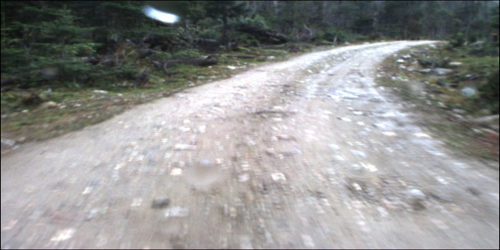
\includegraphics[width=0.3\linewidth]{data/0618.png}
%\caption{fig1}
}
% \quad
\subfigure[0854.png]{
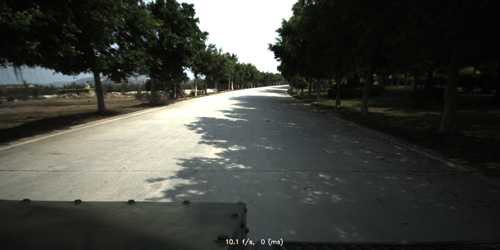
\includegraphics[width=0.3\linewidth]{data/0854.png}
}
% \quad
\subfigure[1066.png]{
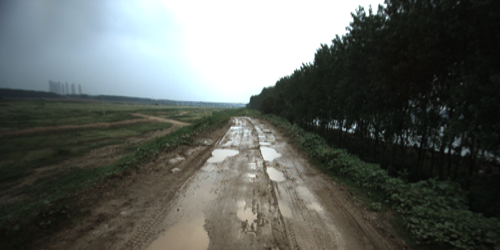
\includegraphics[width=0.3\linewidth]{data/1066.png}
}

\subfigure[0618\_mask.png]{
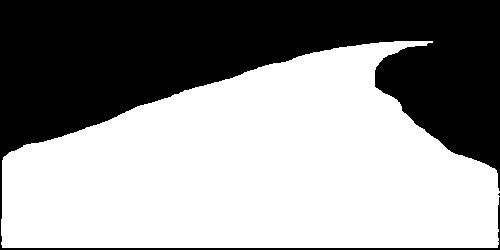
\includegraphics[width=0.3\linewidth]{data/0618_mask.png}
}
% \quad
\subfigure[0854\_mask.png]{
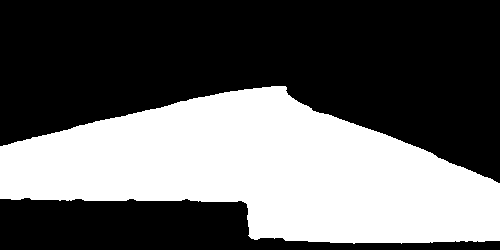
\includegraphics[width=0.3\linewidth]{data/0854_mask.png}
}
% \quad
\subfigure[1066\_mask.png]{
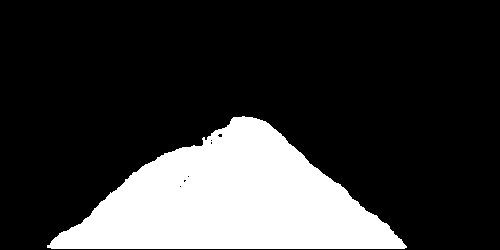
\includegraphics[width=0.3\linewidth]{data/1066_mask.png}
}
\caption{道路mask标签示意图}
\label{fig:mask}
\end{figure}





\subsection{数据预处理:滤波}
在先前的实验中,我们发现在分割结果中,总是会有一些噪点,经过分析,我们发现:道路通常是较为亮的点,即RGB的值均比较高的点,而在非道路中,也可能存在若干点亮度也较高,其与道路样本更加接近,使得可能把一些小的孤立点分割为道路;另一方面,道路中也存在一些颜色较暗的点,其与非道路样本更加接近,使得道路上的一些暗点可能被分割为非道路。
\par
为此,我们计划采用滤波的方式,对原始图像进行预处理。一方面,\textbf{非道路的亮点}会与周围的非道路样本更为接近,降低其被分割为道路的可能性;另一方面,\textbf{道路的暗点}会与周围的道路样本更加接近,增加其被分割为道路的可能性。
\par
在实验中,采用的滤波方式有\textbf{中值滤波}、\textbf{均值滤波}、\textbf{高斯滤波}、\textbf{双边滤波}、\textbf{均值迁移滤波},我们设置的滤波参数如\autoref{tab:滤波实验参数设置}所示,原先我们计划对于滤波设置不同的参数,对不同滤波参数也进行比较,考虑到实验量较大,且本次实验的核心不在于此,因此,我们精心为每一种滤波仅挑选了一组参数进行实验。

\begin{table}[!htbp]

\caption{滤波实验参数设置}
    \centering
    \begin{tabular}{ll}
    \hline
        \textbf{方法} & \textbf{参数设置} \\
        \hline
        中值滤波  & ksize=5 \\
     	
        均值滤波 & ksize=(5,5) \\
        
        高斯滤波  & ksize=(5,5) \\
        
        双边滤波  & d=9, sigmaColor=75, sigmaSpace=75 \\
        
        均值迁移滤波  & sp=10, sr=50 \\
        \hline
    \end{tabular}
    \label{tab:滤波实验参数设置}
\end{table}


\begin{figure}[htbp]
  \centering
  \subfigure[0618.png原图]{
  	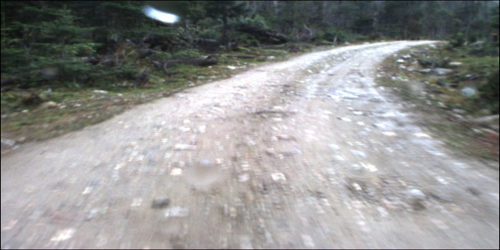
\includegraphics[width=0.3\linewidth]{data/0618.png}
  }
  \subfigure[0854.png原图]{
	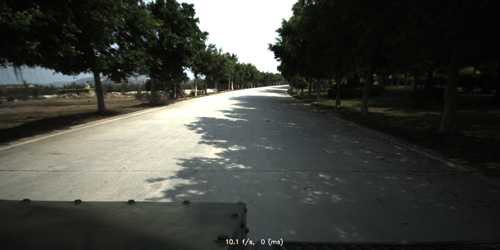
\includegraphics[width=0.3\linewidth]{data/0854.png}
}
  \subfigure[1066.png原图]{
	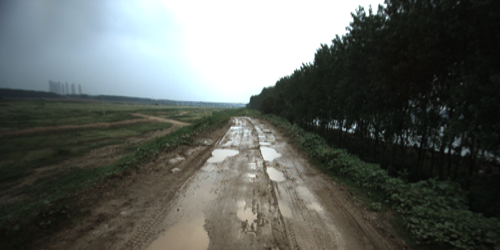
\includegraphics[width=0.3\linewidth]{data/1066.png}
}
  \subfigure[中值滤波]{
	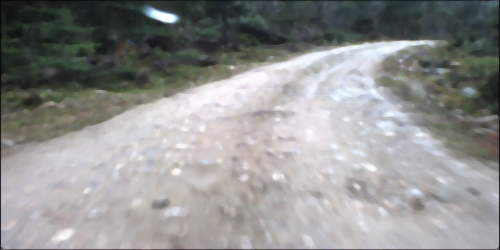
\includegraphics[width=0.3\linewidth]{1_image_processing/median_blur_0618.png}
}
  \subfigure[中值滤波]{
	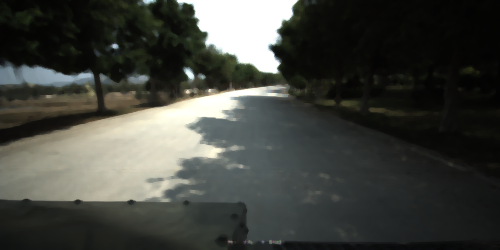
\includegraphics[width=0.3\linewidth]{1_image_processing/median_blur_0854.png}
}
  \subfigure[中值滤波]{
	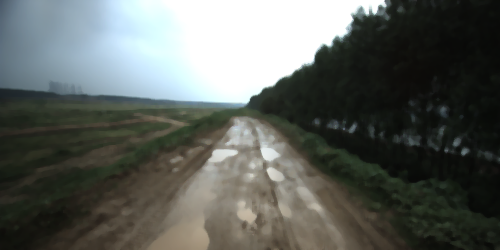
\includegraphics[width=0.3\linewidth]{1_image_processing/median_blur_1066.png}
}
  \subfigure[均值滤波]{
	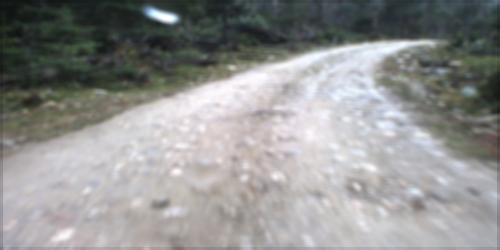
\includegraphics[width=0.3\linewidth]{1_image_processing/average_blur_0618.png}
}
  \subfigure[均值滤波]{
	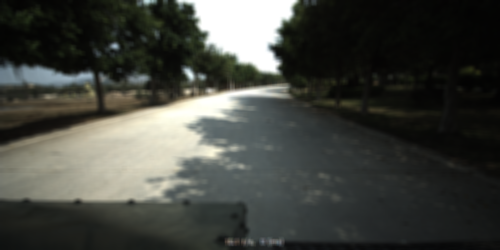
\includegraphics[width=0.3\linewidth]{1_image_processing/average_blur_0854.png}
}
  \subfigure[均值滤波]{
	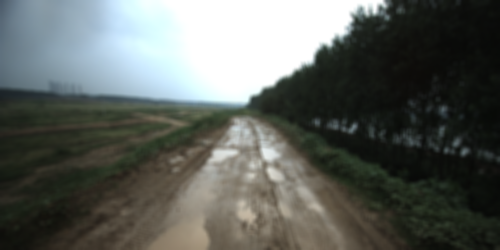
\includegraphics[width=0.3\linewidth]{1_image_processing/average_blur_1066.png}
}
  \subfigure[高斯滤波]{
	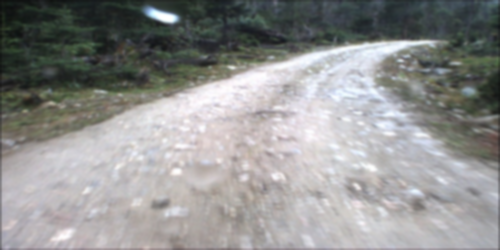
\includegraphics[width=0.3\linewidth]{1_image_processing/gaussian_blur_0618.png}
}
\subfigure[高斯滤波]{
	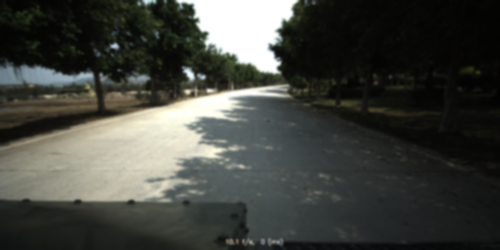
\includegraphics[width=0.3\linewidth]{1_image_processing/gaussian_blur_0854.png}
}
\subfigure[高斯滤波]{
	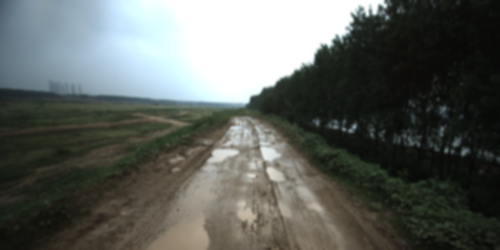
\includegraphics[width=0.3\linewidth]{1_image_processing/gaussian_blur_1066.png}
}
  \subfigure[双边滤波]{
	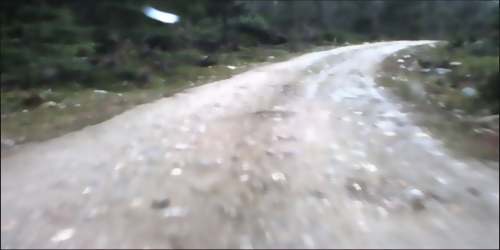
\includegraphics[width=0.3\linewidth]{1_image_processing/bilateral_filter_0618.png}
}
\subfigure[双边滤波]{
	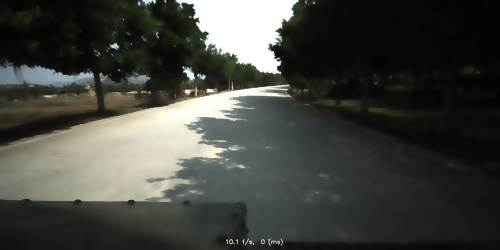
\includegraphics[width=0.3\linewidth]{1_image_processing/bilateral_filter_0854.png}
}
\subfigure[双边滤波]{
	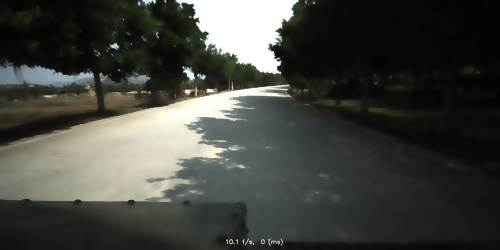
\includegraphics[width=0.3\linewidth]{1_image_processing/bilateral_filter_0854.png}
}
  \subfigure[均值迁移滤波]{
	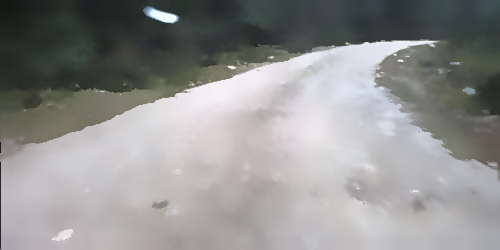
\includegraphics[width=0.3\linewidth]{1_image_processing/mean_shift_filter_0618.png}
}
\subfigure[均值迁移滤波]{
	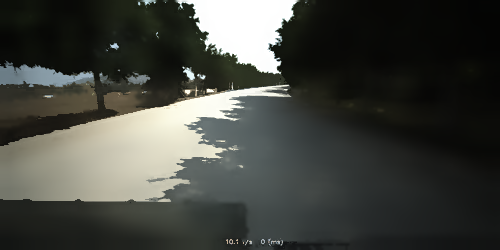
\includegraphics[width=0.3\linewidth]{1_image_processing/mean_shift_filter_0854.png}
}
\subfigure[均值迁移滤波]{
	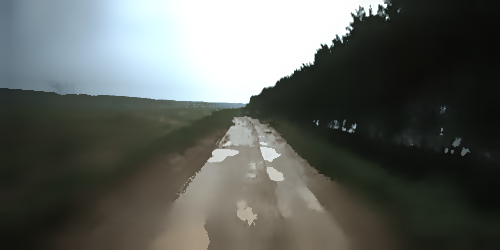
\includegraphics[width=0.3\linewidth]{1_image_processing/mean_shift_filter_1066.png}
}
\caption{原始图像滤波结果}
\label{fig:img_filter}
\end{figure}

\par

\autoref{fig:img_filter}展示了在\autoref{tab:滤波实验参数设置}参数设置下,滤波前后的图像对比,具体滤波形式和图像类型均在图中进行了详尽的描述。


\subsection{特征提取:采用PCA、KPCA、LDA、Dictionary\_Learning}
在本次实验中,我们主要采用了\textbf{主成分分析}(PCA)、\textbf{核主成分分析}(KPCA)、\textbf{线性判别分析}(LDA)和\textbf{字典学习}(Dictionary Learning),在实验中,我们设置不同的参数,具体实验设置如\autoref{tab:特征提取实验参数设置}所示

\begin{table}[!htbp]

\caption{特征提取实验参数设置}
    \centering
    \begin{tabular}{ll}
    \hline
        \textbf{方法} & \textbf{参数设置} \\
        \hline
        Original RGB & None \\
        
        PCA  & n\_components=1,2 \\
        
        KPCA & n\_components=1,2 \\
          & kernel=rbf, poly, sigmoid, cosine \\
          
        LDA  & n\_components=1 \\
        
        Dictionary Learning  & n\_components=1,2 \\
        \hline
    \end{tabular}
    \label{tab:特征提取实验参数设置}
\end{table}

\par
LDA的参数n\_components只能为1,这是因为其在运算中$n\_components \le \min (feaures, n\_classes)$
\par
通过计算,我们可以得出,总共对$1+2+2\times 4 +1+2=14$组特征提取参数进行实验对比。加之前面有5种滤波方式,那么总共有$5\times 14=70$种不同的实验设置。


\subsection{流形学习方法:评估特征提取效果}
在流形学习中,我们采用t-SNE,ISOMAP,lle三种方法进行可视化特征提取效果的可视化展示,由于sklearn是在CPU条件下运行,运算速度特别慢,因此对于这三种方法,我们只针对训练集数据的特征提取效果进行可视化展示。
\par
\textbf{流形学习库的调研}
通过查阅资料,我们发现关于如何高效使用t-SNE的网站{\href{https://distill.pub/2016/misread-tsne}{\textcolor{red}{(How to Use t-SNE Effectively)}},在这个网站中,可以探究不同样本分布情况下,不同参数对于t-SNE的效果展现。
\par
在后续的调研中,我们发现前人在t-SNE的加速上做了很多工作,我们在github上找到了\href{https://github.com/CannyLab/tsne-cuda}{\textcolor{red}{tsne-cuda库}},该库对于t-SNE进行了显著的加速,加速效果如\autoref{fig:tsnecuda}所示
\begin{figure}[htbp]
	\centering
	\subfigure{
		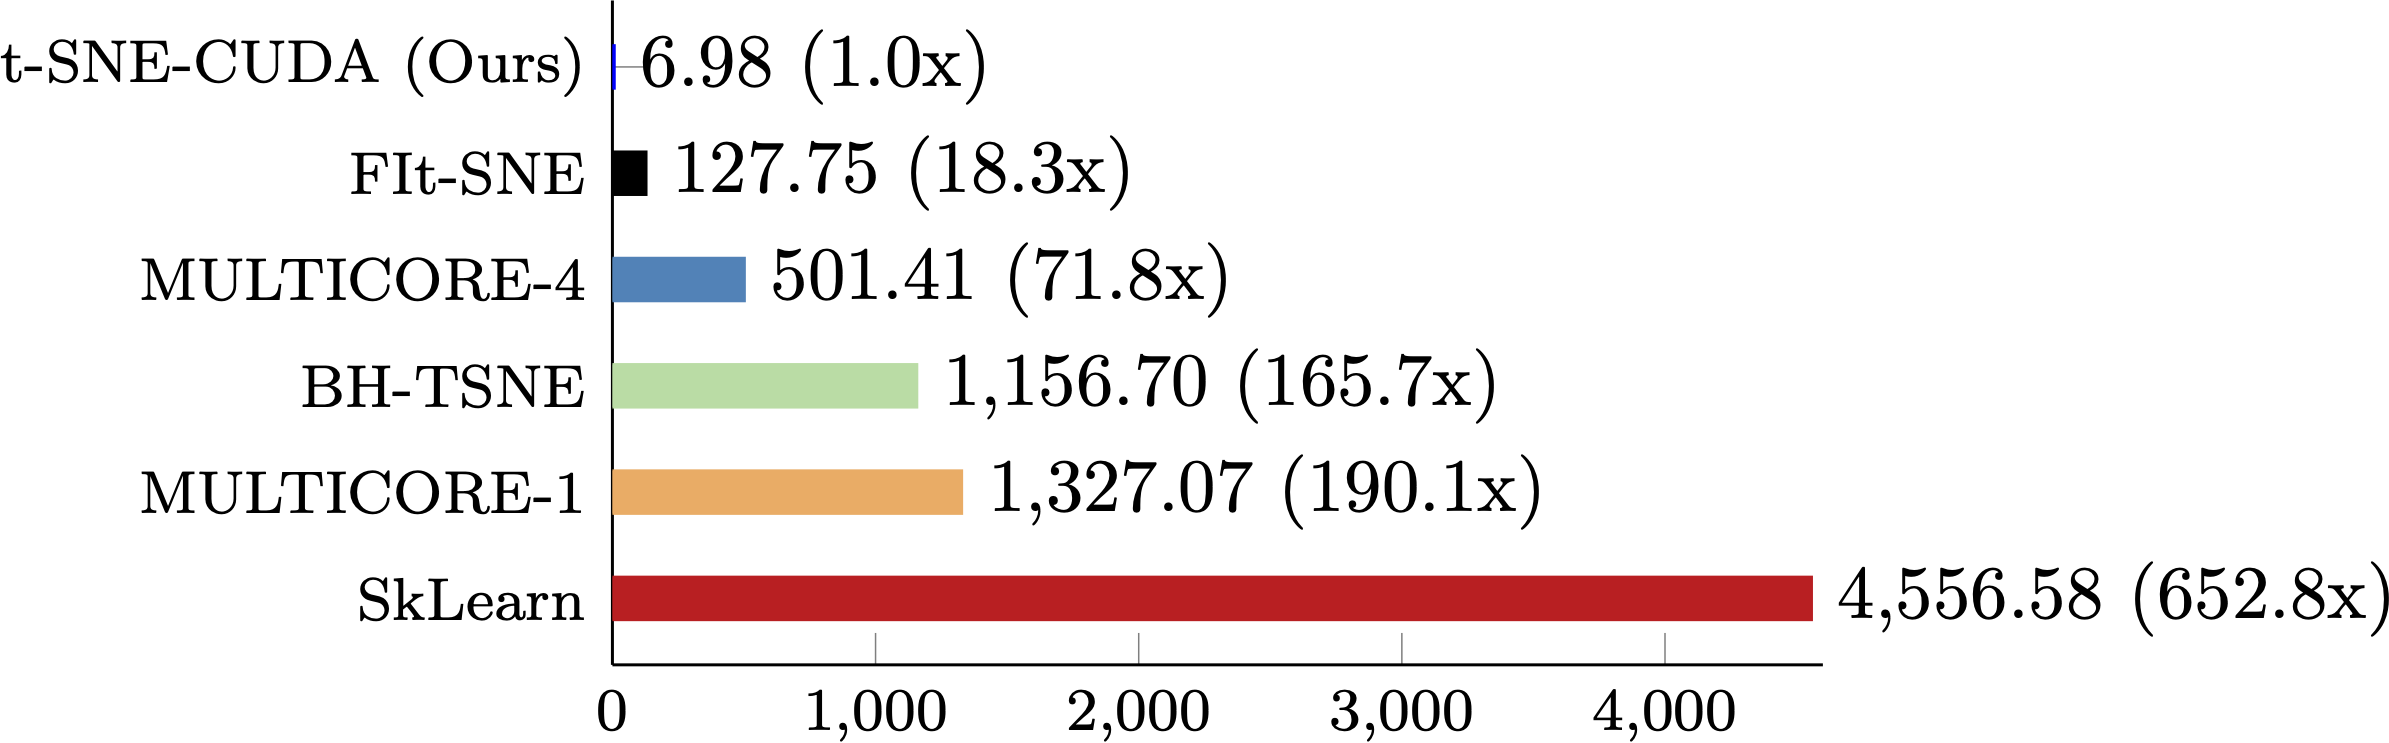
\includegraphics[width=.8\linewidth]{pic/mnist_speedup.png}
}
	\subfigure{
		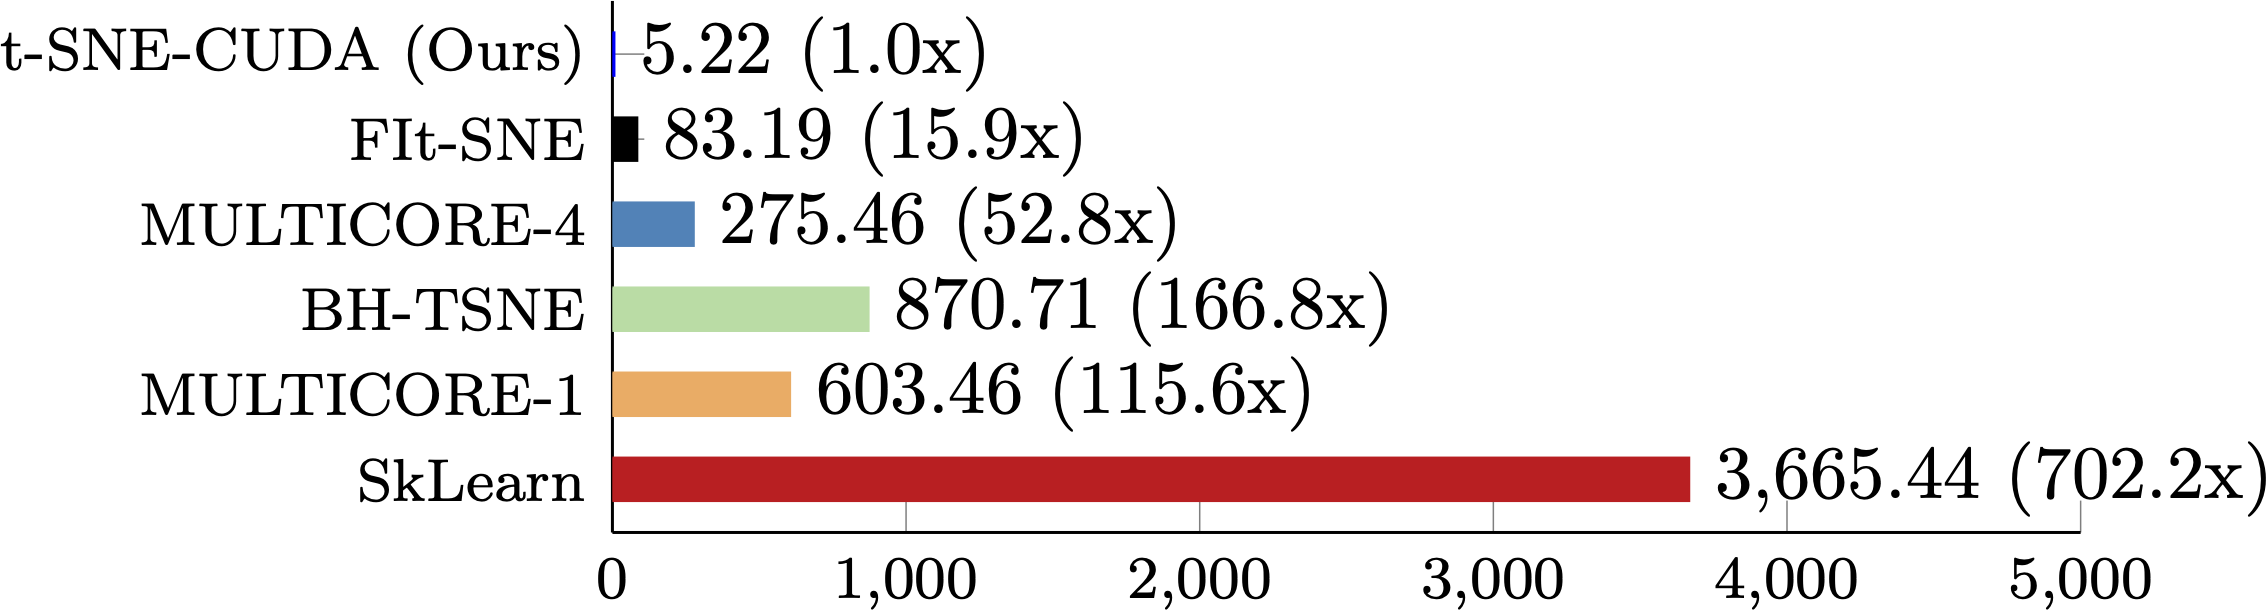
\includegraphics[width=.8\linewidth]{pic/cifar_speedup.png}
	}
	\caption{tsnecuda在MINIST和CIFAR数据集上与其他库运算速度的对比}
	\label{fig:tsnecuda}
\end{figure}

\par
原本以为,可以采用tsnecuda进行加速,但是tsnecuda存在很多问题,其中之一就是不能用pca作为初始化。通过本地的实验对比,我们发现其效果远不如sklearn。从\autoref{fig:tsnecuda缺点}中,我们不难发现,sklearn上的效果明显要优于tsnecuda。
\begin{figure}[htbp]
	\centering
	\subfigure[sklearn上的结果]{
		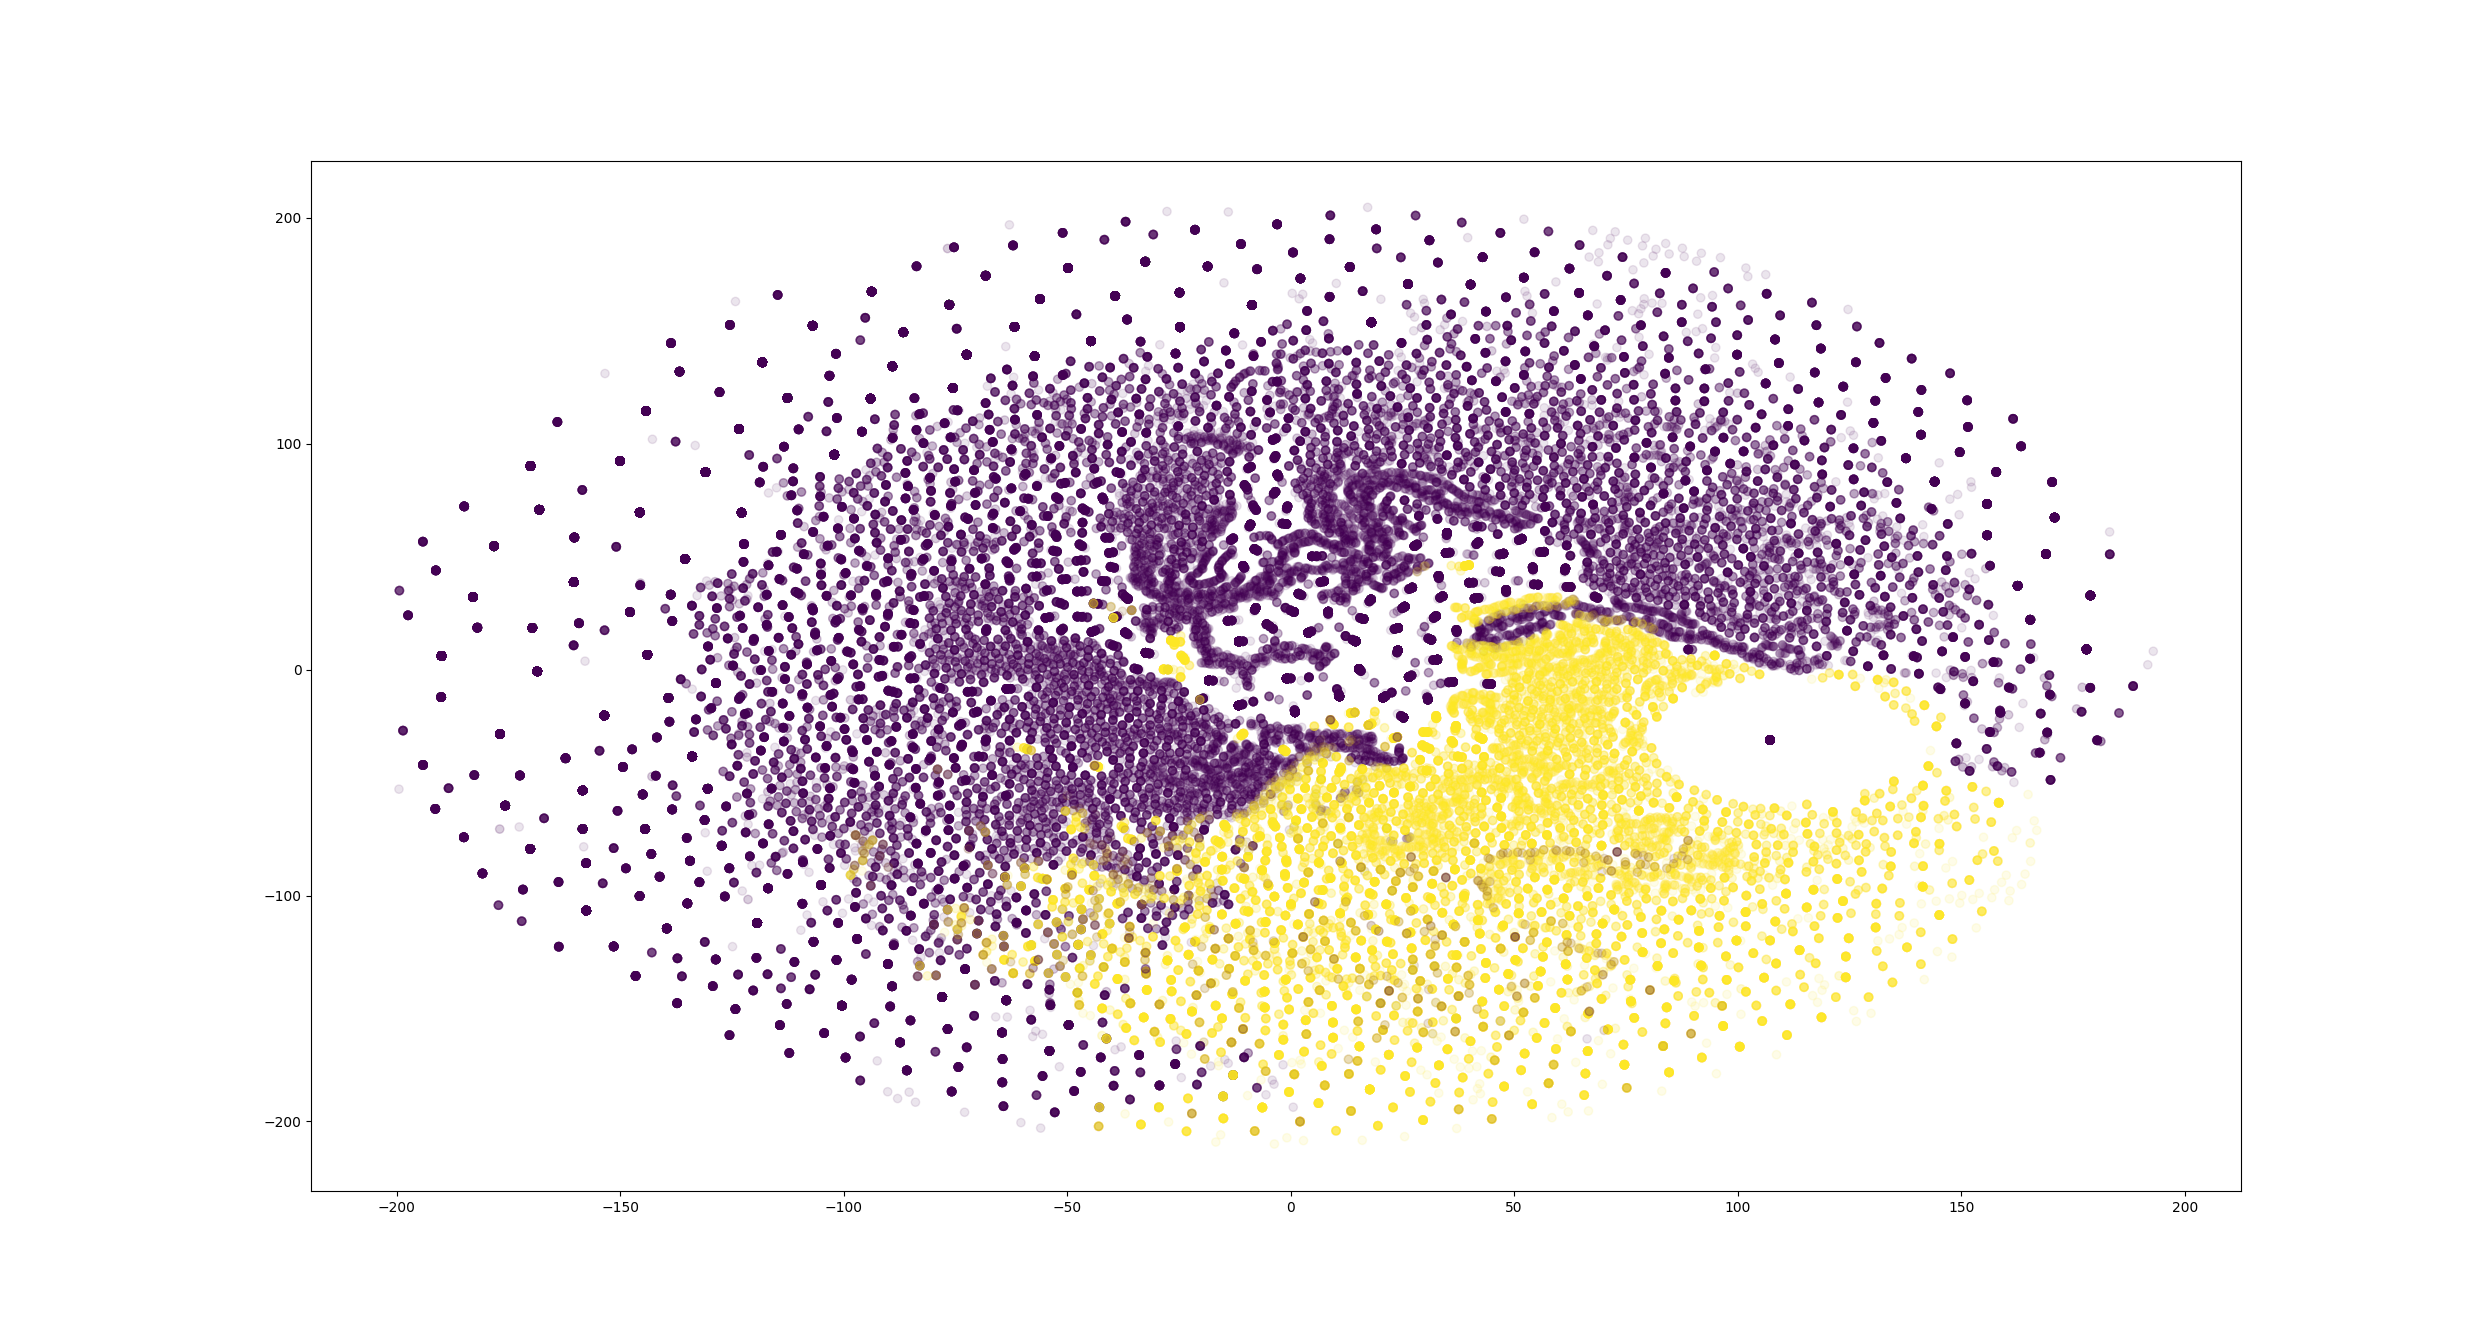
\includegraphics[width=.45\linewidth, trim=30 30 30 30, clip]{pic/sklearn_res.png}
	}
	\subfigure[tsnecuda上的结果]{
		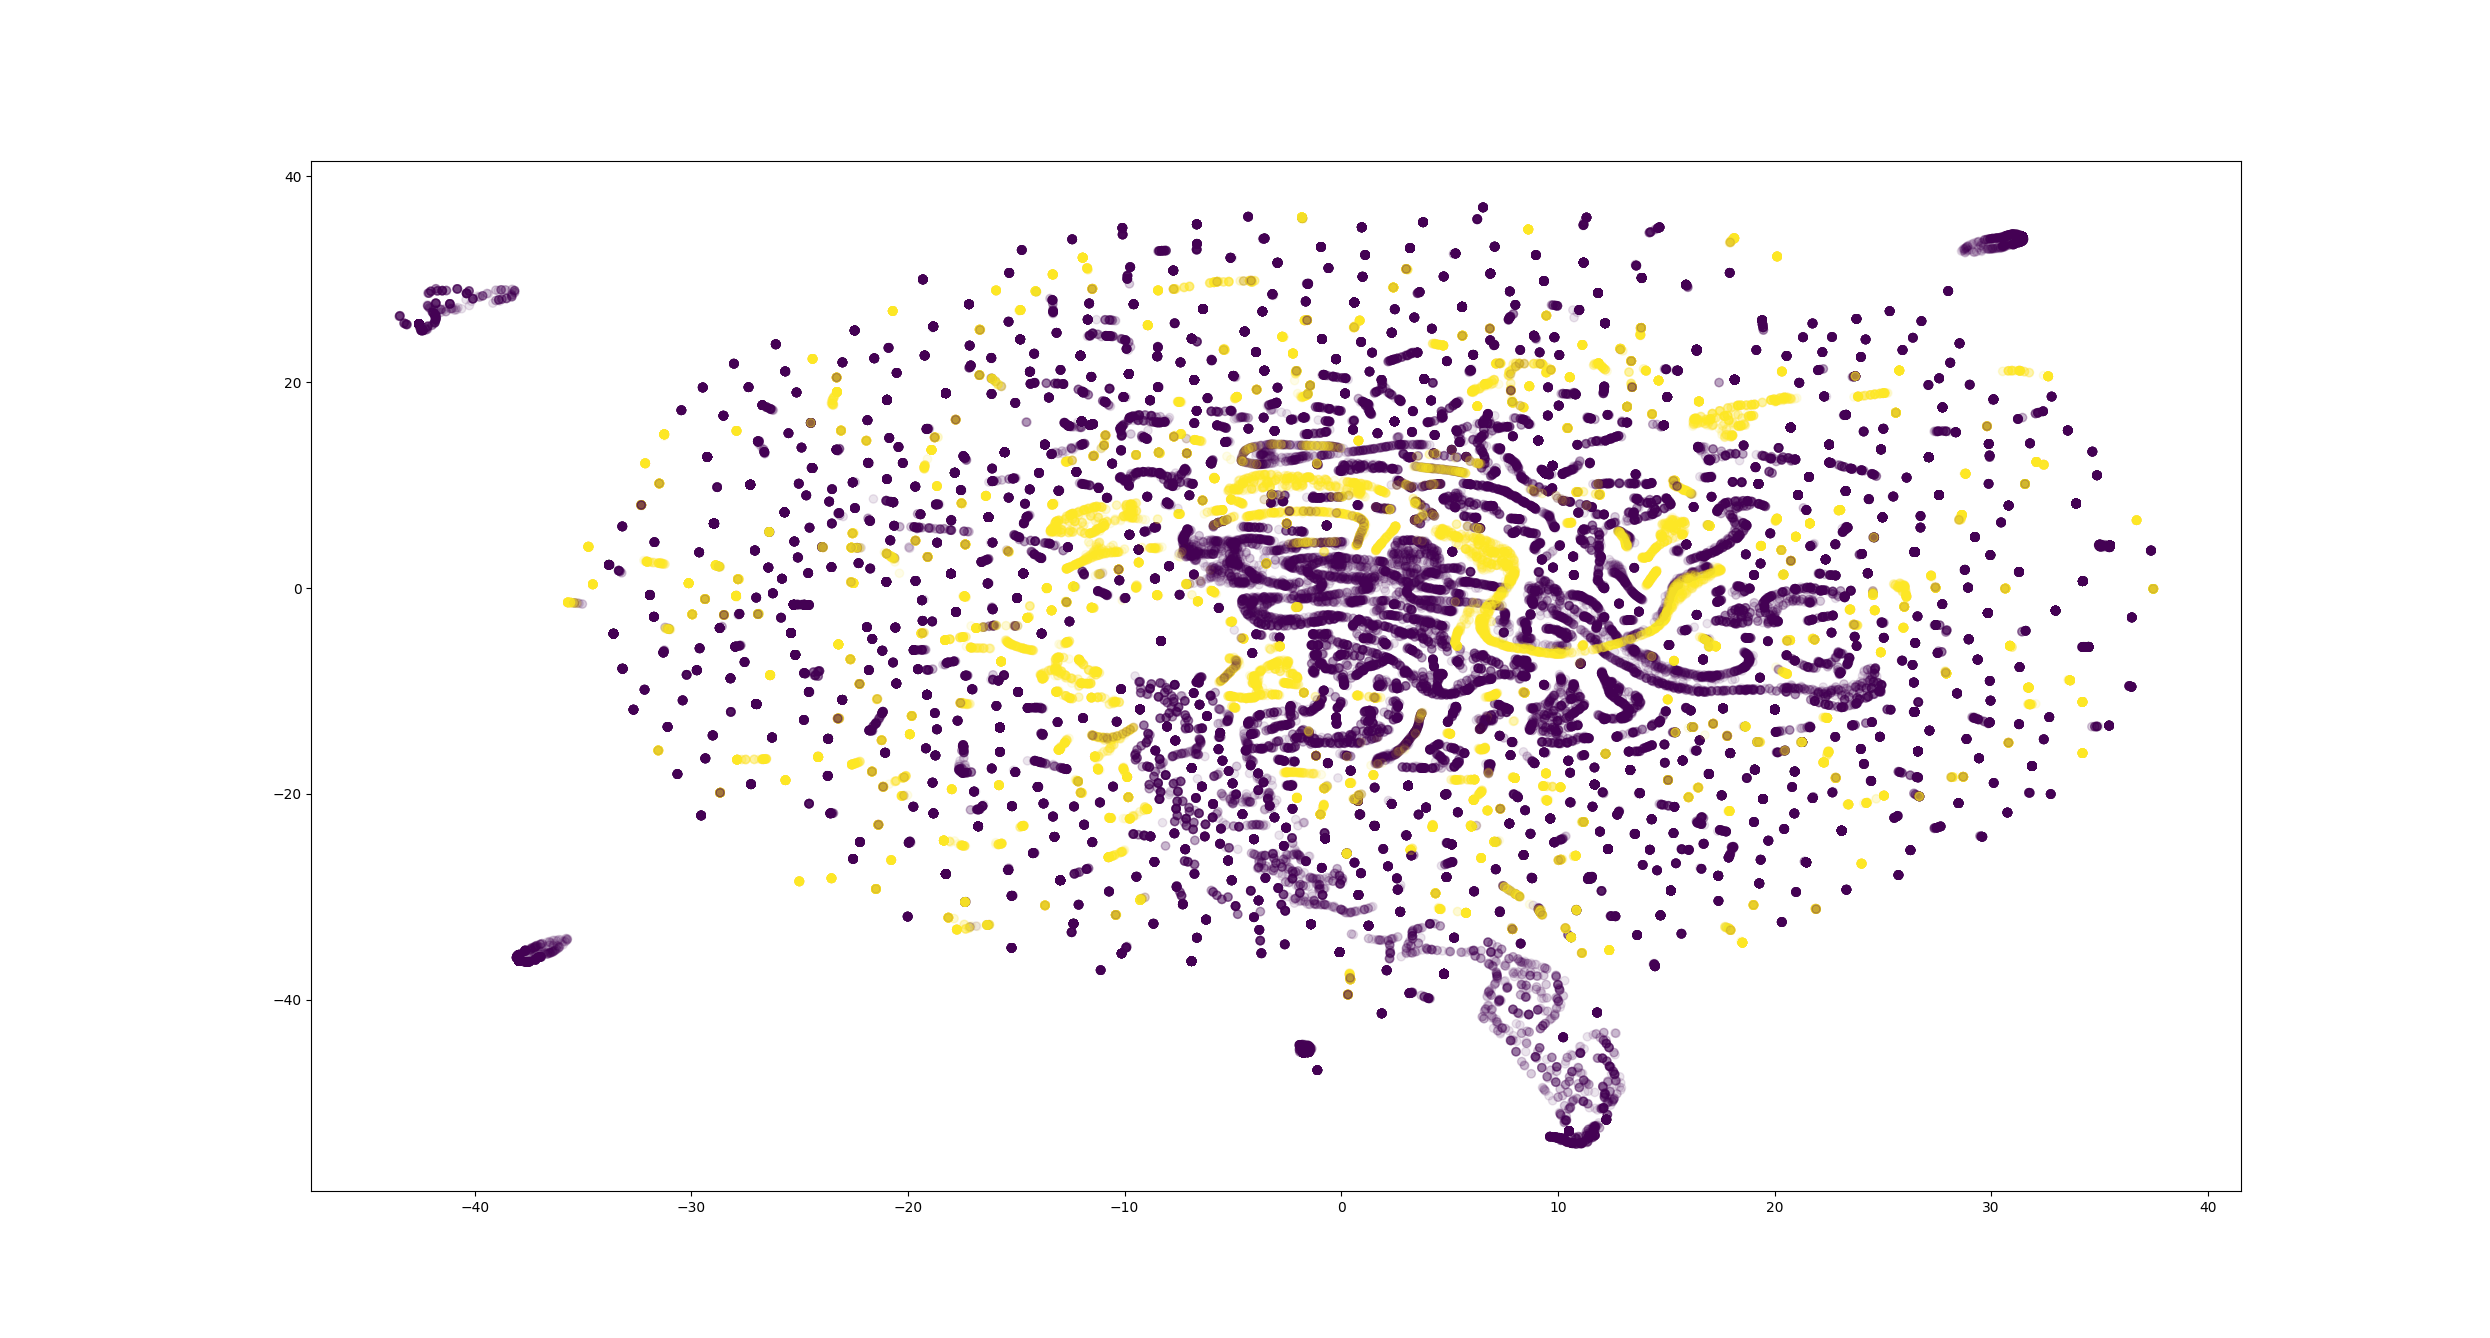
\includegraphics[width=.45\linewidth, trim=30 30 30 30, clip]{pic/tsnecuda_res.png}
	}
	\caption{sklearn和tsnecuda结果对比}
	\label{fig:tsnecuda缺点}
\end{figure}

从\autoref{fig:tsnecuda缺点}中,我们发现,sklearn上能够明显分出紫色和黄色两个类别,但是tsnecuda上,黄色和紫色混杂在了一起,区分的效果明显差于前者。

\par
抛弃了tsnecuda之后,通过调研,我们又发现了\href{https://github.com/rapidsai/cuml}{\textcolor{red}{cuML库}},cuML是一套实现机器学习算法和数学原语函数的库,与其他RAPIDS项目共享兼容的api。cuML使数据科学家、研究人员和软件工程师能够在gpu上运行传统的表格式ML任务,而无需深入CUDA编程的细节。对于大型数据集,这些基于gpu的实现可以比CPU实现快10-50倍。

\textbf{使用sklearn库完成t-SNE,ISOMAP,lle}
%\paragraph{使用sklearn库完成t-SNE,ISOMAP,lle}
基于前面所讲述的,我们先利用sklearn库,采用t-SNE,ISOMAP,lle三种方法进行可视化特征提取效果的可视化展示。我们现在总共具有三个维度:滤波方式、特征提取方式、流形学习方式,不易直接展示。首先我们先看滤波方式和流形学习之间的关系。
\begin{figure}[!h]
	\centering
	\subfigure[中值滤波]{
	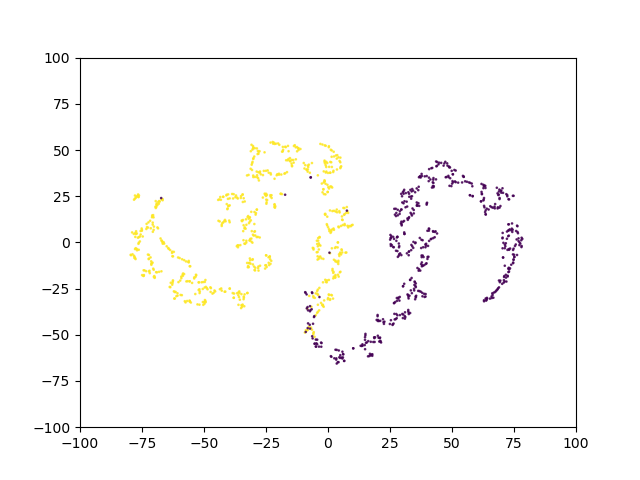
\includegraphics[width=.16\linewidth]{../output/06182/median_blur/original_feature/feature_1_tsne.png}
	}
	\subfigure[均值滤波]{
	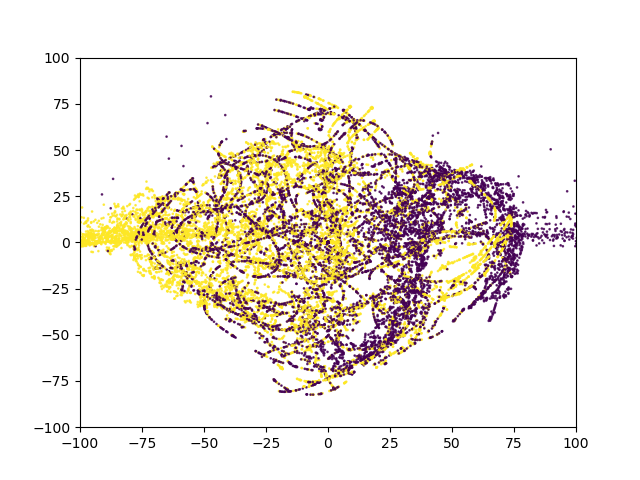
\includegraphics[width=.16\linewidth]{../output/06182/average_blur/original_feature/feature_1_tsne.png}
}
	\subfigure[高斯滤波]{
	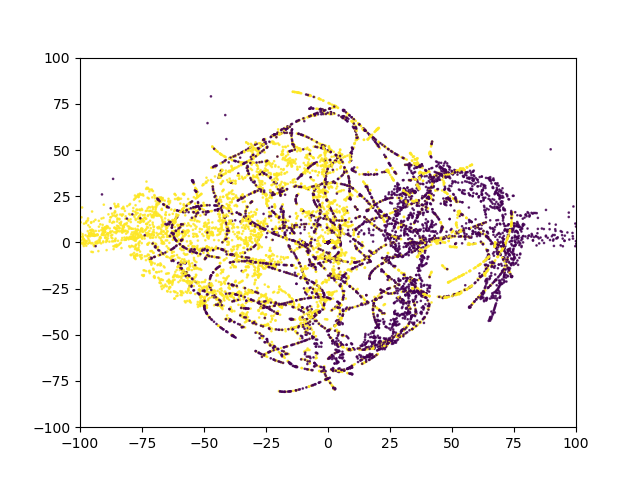
\includegraphics[width=.16\linewidth]{../output/06182/gaussian_blur/original_feature/feature_1_tsne.png}
}
	\subfigure[双边滤波]{
	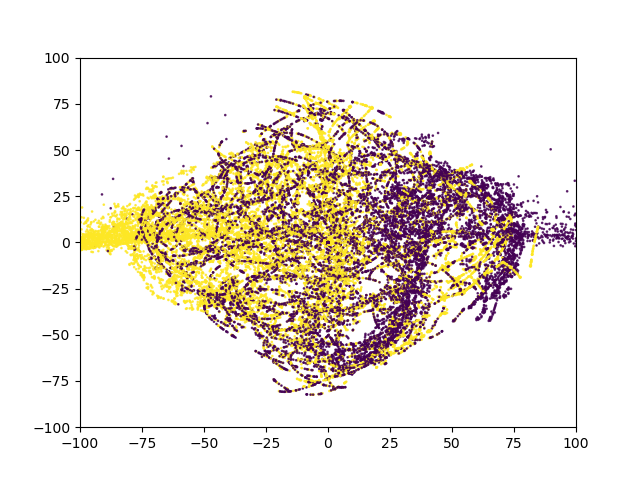
\includegraphics[width=.16\linewidth]{../output/06182/bilateral_filter/original_feature/feature_1_tsne.png}
}
	\subfigure[均值迁移滤波]{
	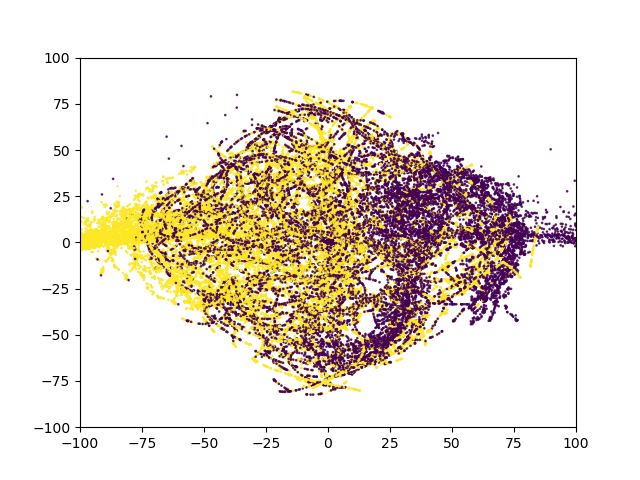
\includegraphics[width=.16\linewidth]{../output/06182/mean_shift_filter/original_feature/feature_1_tsne.png}
}

\subfigure[中值滤波]{
	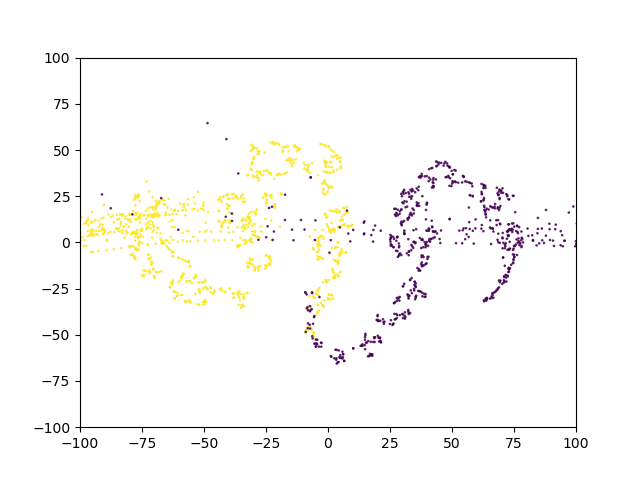
\includegraphics[width=.16\linewidth]{../output/06182/median_blur/original_feature/feature_1_isomap.png}
}
\subfigure[均值滤波]{
	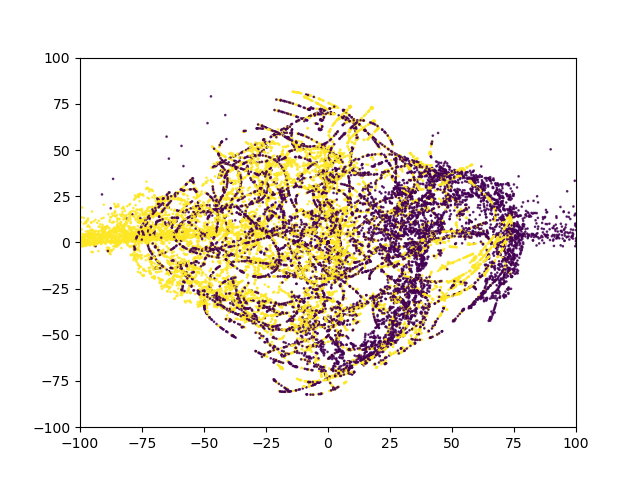
\includegraphics[width=.16\linewidth]{../output/06182/average_blur/original_feature/feature_1_isomap.png}
}
\subfigure[高斯滤波]{
	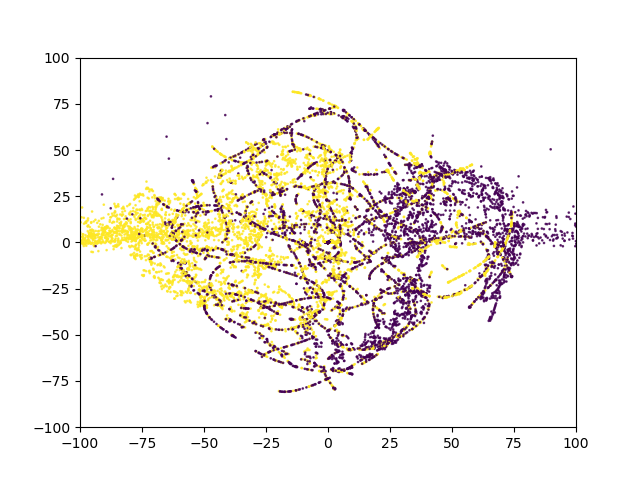
\includegraphics[width=.16\linewidth]{../output/06182/gaussian_blur/original_feature/feature_1_isomap.png}
}
\subfigure[双边滤波]{
	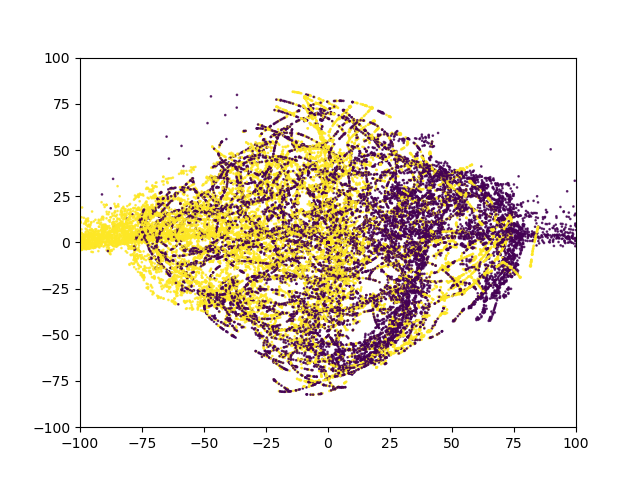
\includegraphics[width=.16\linewidth]{../output/06182/bilateral_filter/original_feature/feature_1_isomap.png}
}
\subfigure[均值迁移滤波]{
	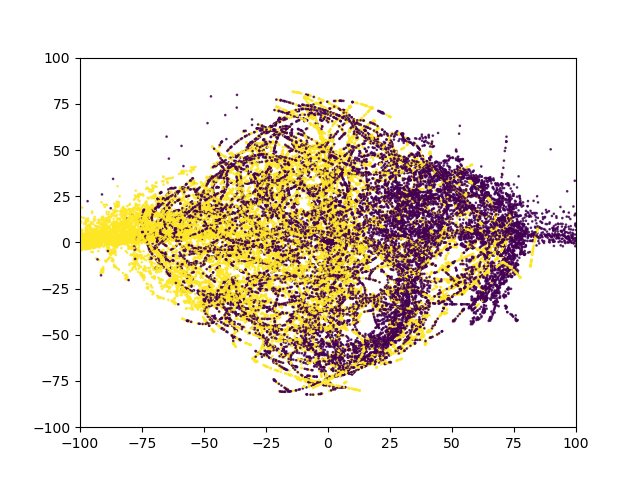
\includegraphics[width=.16\linewidth]{../output/06182/mean_shift_filter/original_feature/feature_1_isomap.png}
}

\subfigure[中值滤波]{
	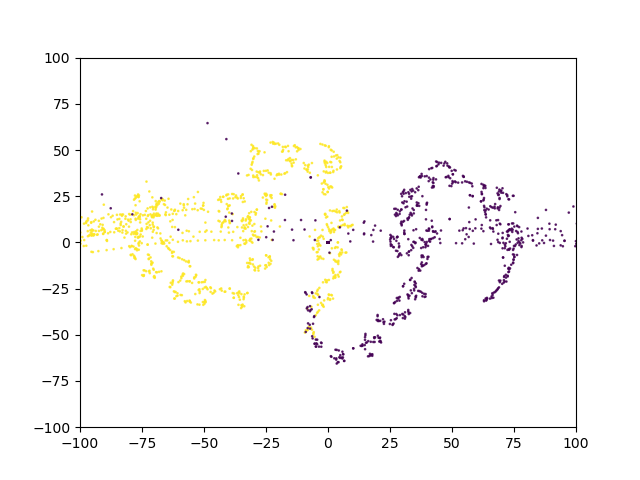
\includegraphics[width=.16\linewidth]{../output/06182/median_blur/original_feature/feature_1_lle.png}
}
\subfigure[均值滤波]{
	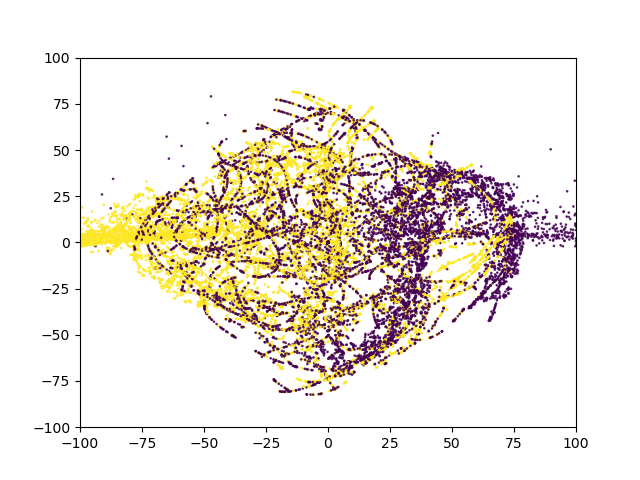
\includegraphics[width=.16\linewidth]{../output/06182/average_blur/original_feature/feature_1_lle.png}
}
\subfigure[高斯滤波]{
	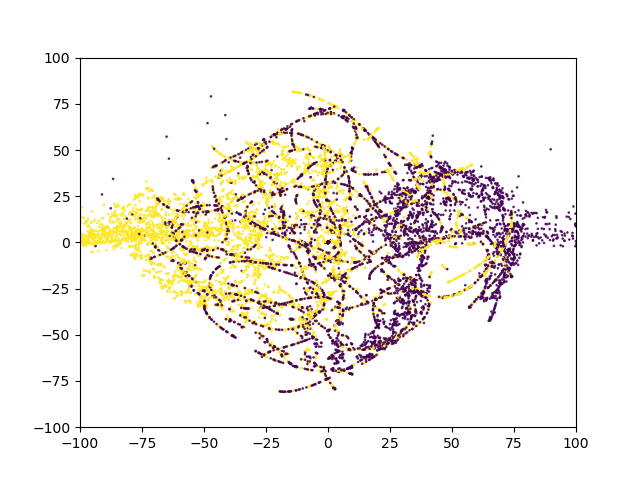
\includegraphics[width=.16\linewidth]{../output/06182/gaussian_blur/original_feature/feature_1_lle.png}
}
\subfigure[双边滤波]{
	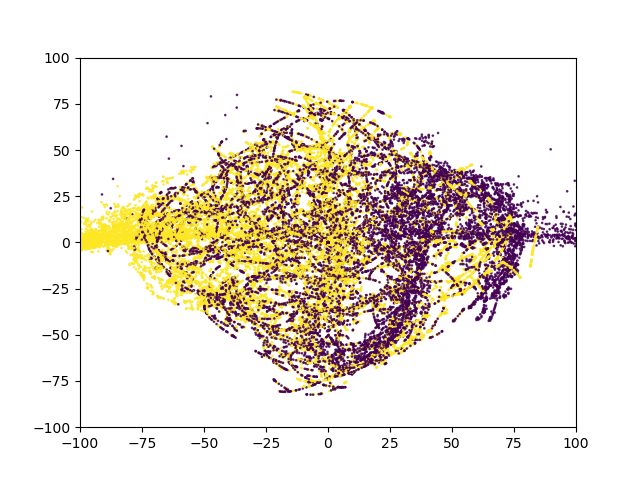
\includegraphics[width=.16\linewidth]{../output/06182/bilateral_filter/original_feature/feature_1_lle.png}
}
\subfigure[均值迁移滤波]{
	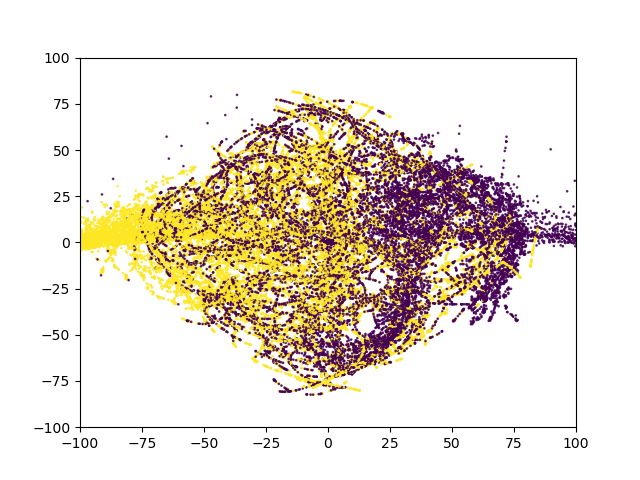
\includegraphics[width=.16\linewidth]{../output/06182/mean_shift_filter/original_feature/feature_1_lle.png}
}
\caption{0618.png平滤波方式与流形学习之间的关系}
\label{fig:滤波方式与流形学习之间的关系0618}
\end{figure}


\begin{figure}[!h]
	\centering
	\subfigure[中值滤波]{
		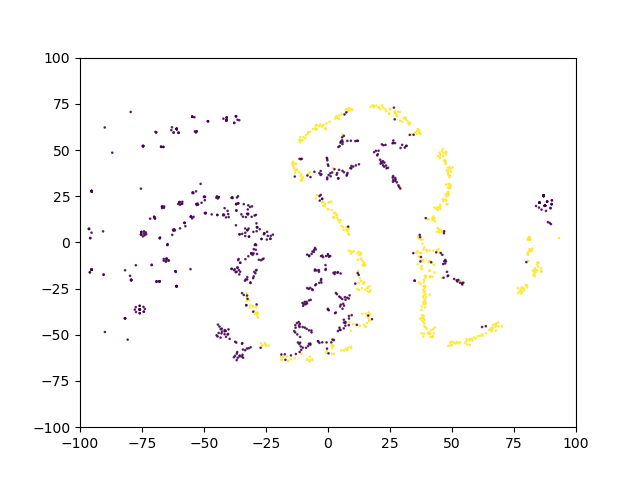
\includegraphics[width=.16\linewidth]{../output/08542/median_blur/original_feature/feature_1_tsne.png}
	}
	\subfigure[均值滤波]{
		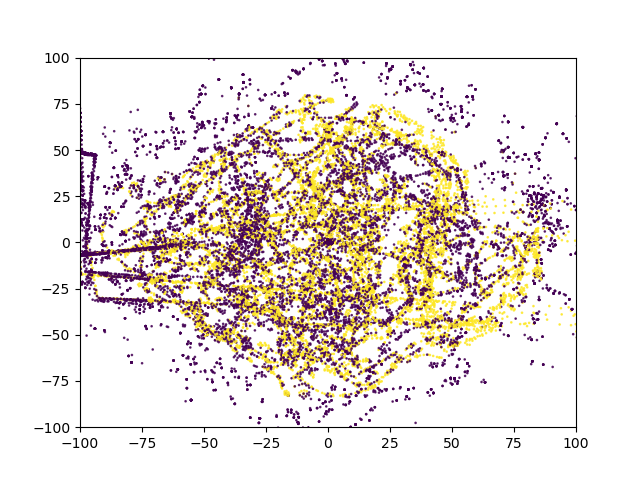
\includegraphics[width=.16\linewidth]{../output/08542/average_blur/original_feature/feature_1_tsne.png}
	}
	\subfigure[高斯滤波]{
		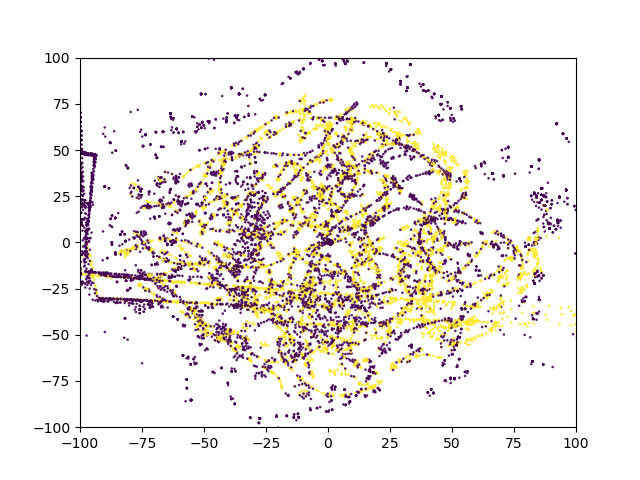
\includegraphics[width=.16\linewidth]{../output/08542/gaussian_blur/original_feature/feature_1_tsne.png}
	}
	\subfigure[双边滤波]{
		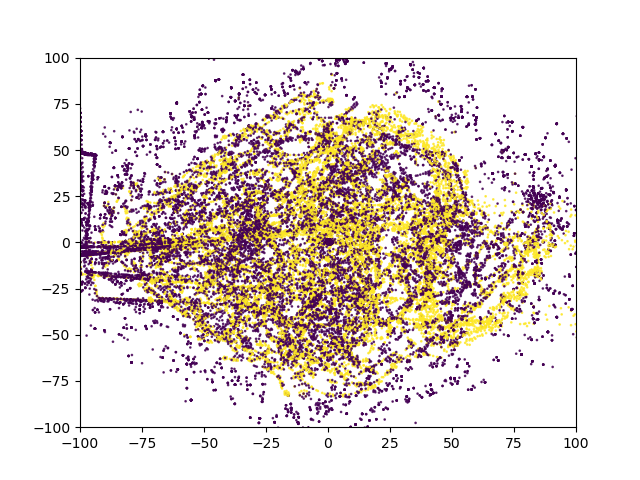
\includegraphics[width=.16\linewidth]{../output/08542/bilateral_filter/original_feature/feature_1_tsne.png}
	}
	\subfigure[均值迁移滤波]{
		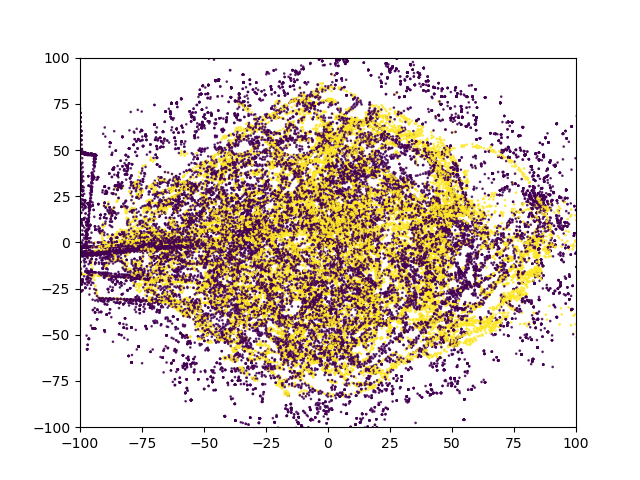
\includegraphics[width=.16\linewidth]{../output/08542/mean_shift_filter/original_feature/feature_1_tsne.png}
	}
	
	\subfigure[中值滤波]{
		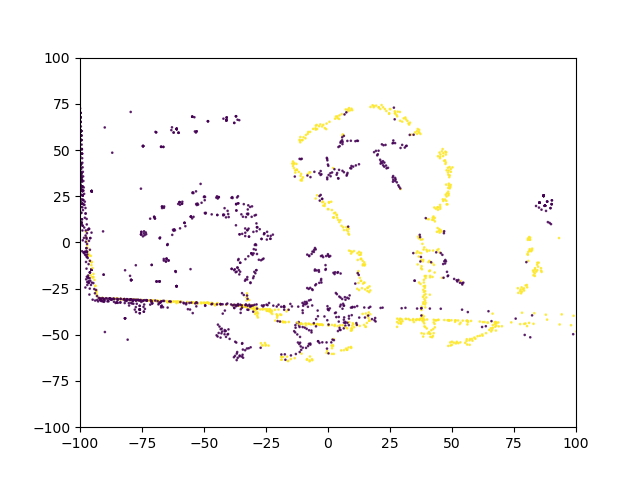
\includegraphics[width=.16\linewidth]{../output/08542/median_blur/original_feature/feature_1_isomap.png}
	}
	\subfigure[均值滤波]{
		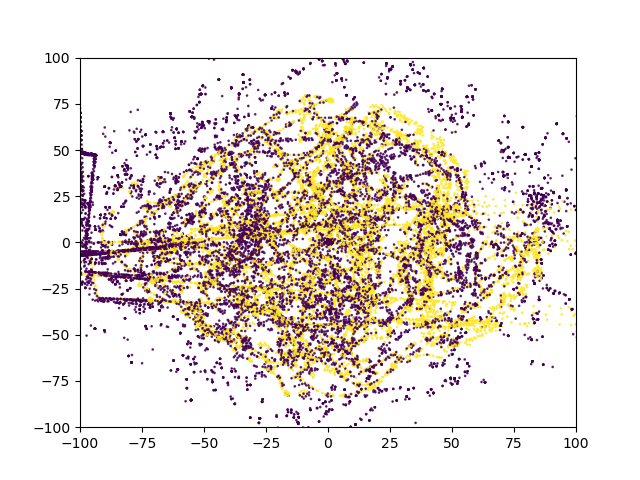
\includegraphics[width=.16\linewidth]{../output/08542/average_blur/original_feature/feature_1_isomap.png}
	}
	\subfigure[高斯滤波]{
		\includegraphics[width=.16\linewidth]{../output/08542/gaussian_blur/original_feature/feature_1_isomap.png}
	}
	\subfigure[双边滤波]{
		\includegraphics[width=.16\linewidth]{../output/08542/bilateral_filter/original_feature/feature_1_isomap.png}
	}
	\subfigure[均值迁移滤波]{
		\includegraphics[width=.16\linewidth]{../output/08542/mean_shift_filter/original_feature/feature_1_isomap.png}
	}
	
	\subfigure[中值滤波]{
		\includegraphics[width=.16\linewidth]{../output/08542/median_blur/original_feature/feature_1_lle.png}
	}
	\subfigure[均值滤波]{
		\includegraphics[width=.16\linewidth]{../output/08542/average_blur/original_feature/feature_1_lle.png}
	}
	\subfigure[高斯滤波]{
		\includegraphics[width=.16\linewidth]{../output/08542/gaussian_blur/original_feature/feature_1_lle.png}
	}
	\subfigure[双边滤波]{
		\includegraphics[width=.16\linewidth]{../output/08542/bilateral_filter/original_feature/feature_1_lle.png}
	}
	\subfigure[均值迁移滤波]{
		\includegraphics[width=.16\linewidth]{../output/08542/mean_shift_filter/original_feature/feature_1_lle.png}
	}
	\caption{0854.png滤波方式与流形学习之间的关系}
	\label{fig:滤波方式与流形学习之间的关系0854}
\end{figure}


\begin{figure}[!h]
	\centering
	\subfigure[中值滤波]{
		\includegraphics[width=.16\linewidth]{../output/10662/median_blur/original_feature/feature_1_tsne.png}
	}
	\subfigure[均值滤波]{
		\includegraphics[width=.16\linewidth]{../output/10662/average_blur/original_feature/feature_1_tsne.png}
	}
	\subfigure[高斯滤波]{
		\includegraphics[width=.16\linewidth]{../output/10662/gaussian_blur/original_feature/feature_1_tsne.png}
	}
	\subfigure[双边滤波]{
		\includegraphics[width=.16\linewidth]{../output/10662/bilateral_filter/original_feature/feature_1_tsne.png}
	}
	\subfigure[均值迁移滤波]{
		\includegraphics[width=.16\linewidth]{../output/10662/mean_shift_filter/original_feature/feature_1_tsne.png}
	}
	
	\subfigure[中值滤波]{
		\includegraphics[width=.16\linewidth]{../output/10662/median_blur/original_feature/feature_1_isomap.png}
	}
	\subfigure[均值滤波]{
		\includegraphics[width=.16\linewidth]{../output/10662/average_blur/original_feature/feature_1_isomap.png}
	}
	\subfigure[高斯滤波]{
		\includegraphics[width=.16\linewidth]{../output/10662/gaussian_blur/original_feature/feature_1_isomap.png}
	}
	\subfigure[双边滤波]{
		\includegraphics[width=.16\linewidth]{../output/10662/bilateral_filter/original_feature/feature_1_isomap.png}
	}
	\subfigure[均值迁移滤波]{
		\includegraphics[width=.16\linewidth]{../output/10662/mean_shift_filter/original_feature/feature_1_isomap.png}
	}
	
	\subfigure[中值滤波]{
		\includegraphics[width=.16\linewidth]{../output/10662/median_blur/original_feature/feature_1_lle.png}
	}
	\subfigure[均值滤波]{
		\includegraphics[width=.16\linewidth]{../output/10662/average_blur/original_feature/feature_1_lle.png}
	}
	\subfigure[高斯滤波]{
		\includegraphics[width=.16\linewidth]{../output/10662/gaussian_blur/original_feature/feature_1_lle.png}
	}
	\subfigure[双边滤波]{
		\includegraphics[width=.16\linewidth]{../output/10662/bilateral_filter/original_feature/feature_1_lle.png}
	}
	\subfigure[均值迁移滤波]{
		\includegraphics[width=.16\linewidth]{../output/10662/mean_shift_filter/original_feature/feature_1_lle.png}
	}
	\caption{1066.png滤波方式与流形学习之间的关系}
	\label{fig:滤波方式与流形学习之间的关系1066}
\end{figure}


\autoref{fig:滤波方式与流形学习之间的关系0618}-\ref{fig:滤波方式与流形学习之间的关系1066}展示了5种滤波方式与流形学习之间的关系,从上至下分别是t-SNE,ISOMAP,lle三种方法,我们发现滤波方式对于流形学习的结果,其实也就是特征提取的结果,有一定的影响,中值滤波的效果要优于其他的方式,但是也有可能是流形学习没有做到很好的分类效果。横向上来看,t-SNE,ISOMAP,lle三种方法差别不大,后两者的分类效果要稍微差于t-SNE,但是总体来讲,差别不大。
\par

下面我们再比较特征提取与流形学习之间的关系,这里我们选取中值滤波方式。



\begin{figure}[!h]
	\centering
	\subfigure{
		\includegraphics[width=.30\linewidth]{../output/06182/median_blur/original_feature/feature_1_tsne.png}
}
	\subfigure{
	\includegraphics[width=.30\linewidth]{../output/06182/median_blur/original_feature/feature_1_isomap.png}
}
	\subfigure{
	\includegraphics[width=.30\linewidth]{../output/06182/median_blur/original_feature/feature_1_lle.png}
}
\vspace{-0.3cm}
	\subfigure{
	\includegraphics[width=.30\linewidth]{../output/06182/median_blur/pca_feature/feature_2_tsne.png}
}
\subfigure{
	\includegraphics[width=.30\linewidth]{../output/06182/median_blur/pca_feature/feature_2_isomap.png}
}
\subfigure{
	\includegraphics[width=.30\linewidth]{../output/06182/median_blur/pca_feature/feature_2_lle.png}
}
\vspace{-0.3cm}
	\subfigure{
	\includegraphics[width=.30\linewidth]{../output/06182/median_blur/kpca_feature/feature_3_tsne.png}
}
\subfigure{
	\includegraphics[width=.30\linewidth]{../output/06182/median_blur/kpca_feature/feature_3_isomap.png}
}
\subfigure{
	\includegraphics[width=.30\linewidth]{../output/06182/median_blur/kpca_feature/feature_3_lle.png}
}
\vspace{-0.3cm}
	\subfigure{
	\includegraphics[width=.30\linewidth]{../output/06182/median_blur/kpca_feature/feature_4_tsne.png}
}
\subfigure{
	\includegraphics[width=.30\linewidth]{../output/06182/median_blur/kpca_feature/feature_4_isomap.png}
}
\subfigure{
	\includegraphics[width=.30\linewidth]{../output/06182/median_blur/kpca_feature/feature_4_lle.png}
}
\vspace{-0.3cm}
	\subfigure{
	\includegraphics[width=.30\linewidth]{../output/06182/median_blur/kpca_feature/feature_5_tsne.png}
}
\subfigure{
	\includegraphics[width=.30\linewidth]{../output/06182/median_blur/kpca_feature/feature_5_isomap.png}
}
\subfigure{
	\includegraphics[width=.30\linewidth]{../output/06182/median_blur/kpca_feature/feature_5_lle.png}
}
\vspace{-0.3cm}
	\subfigure{
	\includegraphics[width=.30\linewidth]{../output/06182/median_blur/dictionary_learning_feature/feature_7_tsne.png}
}
\subfigure{
	\includegraphics[width=.30\linewidth]{../output/06182/median_blur/dictionary_learning_feature/feature_7_isomap.png}
}
\subfigure{
	\includegraphics[width=.30\linewidth]{../output/06182/median_blur/dictionary_learning_feature/feature_7_lle.png}
}
	
	\caption{0618.png特征提取与流形学习之间的关系}
	\label{fig:特征提取与流形学习之间的关系0618}
\end{figure}



\begin{figure}[!h]
	\centering
	\subfigure{
		\includegraphics[width=.30\linewidth]{../output/08542/median_blur/original_feature/feature_1_tsne.png}
	}
	\subfigure{
		\includegraphics[width=.30\linewidth]{../output/08542/median_blur/original_feature/feature_1_isomap.png}
	}
	\subfigure{
		\includegraphics[width=.30\linewidth]{../output/08542/median_blur/original_feature/feature_1_lle.png}
	}
	\vspace{-0.3cm}
	\subfigure{
		\includegraphics[width=.30\linewidth]{../output/08542/median_blur/pca_feature/feature_2_tsne.png}
	}
	\subfigure{
		\includegraphics[width=.30\linewidth]{../output/08542/median_blur/pca_feature/feature_2_isomap.png}
	}
	\subfigure{
		\includegraphics[width=.30\linewidth]{../output/08542/median_blur/pca_feature/feature_2_lle.png}
	}
	\vspace{-0.3cm}
	\subfigure{
		\includegraphics[width=.30\linewidth]{../output/08542/median_blur/kpca_feature/feature_3_tsne.png}
	}
	\subfigure{
		\includegraphics[width=.30\linewidth]{../output/08542/median_blur/kpca_feature/feature_3_isomap.png}
	}
	\subfigure{
		\includegraphics[width=.30\linewidth]{../output/08542/median_blur/kpca_feature/feature_3_lle.png}
	}
	\vspace{-0.3cm}
	\subfigure{
		\includegraphics[width=.30\linewidth]{../output/08542/median_blur/kpca_feature/feature_4_tsne.png}
	}
	\subfigure{
		\includegraphics[width=.30\linewidth]{../output/08542/median_blur/kpca_feature/feature_4_isomap.png}
	}
	\subfigure{
		\includegraphics[width=.30\linewidth]{../output/08542/median_blur/kpca_feature/feature_4_lle.png}
	}
	\vspace{-0.3cm}
	\subfigure{
		\includegraphics[width=.30\linewidth]{../output/08542/median_blur/kpca_feature/feature_5_tsne.png}
	}
	\subfigure{
		\includegraphics[width=.30\linewidth]{../output/08542/median_blur/kpca_feature/feature_5_isomap.png}
	}
	\subfigure{
		\includegraphics[width=.30\linewidth]{../output/08542/median_blur/kpca_feature/feature_5_lle.png}
	}
	\vspace{-0.3cm}
	\subfigure{
		\includegraphics[width=.30\linewidth]{../output/08542/median_blur/dictionary_learning_feature/feature_7_tsne.png}
	}
	\subfigure{
		\includegraphics[width=.30\linewidth]{../output/08542/median_blur/dictionary_learning_feature/feature_7_isomap.png}
	}
	\subfigure{
		\includegraphics[width=.30\linewidth]{../output/08542/median_blur/dictionary_learning_feature/feature_7_lle.png}
	}
	
	\caption{0854.png特征提取与流形学习之间的关系}
	\label{fig:特征提取与流形学习之间的关系0854}
\end{figure}



\begin{figure}[!h]
	\centering
	\subfigure{
		\includegraphics[width=.30\linewidth]{../output/10662/median_blur/original_feature/feature_1_tsne.png}
	}
	\subfigure{
		\includegraphics[width=.30\linewidth]{../output/10662/median_blur/original_feature/feature_1_isomap.png}
	}
	\subfigure{
		\includegraphics[width=.30\linewidth]{../output/10662/median_blur/original_feature/feature_1_lle.png}
	}
	\vspace{-0.3cm}
	\subfigure{
		\includegraphics[width=.30\linewidth]{../output/10662/median_blur/pca_feature/feature_2_tsne.png}
	}
	\subfigure{
		\includegraphics[width=.30\linewidth]{../output/10662/median_blur/pca_feature/feature_2_isomap.png}
	}
	\subfigure{
		\includegraphics[width=.30\linewidth]{../output/10662/median_blur/pca_feature/feature_2_lle.png}
	}
	\vspace{-0.3cm}
	\subfigure{
		\includegraphics[width=.30\linewidth]{../output/10662/median_blur/kpca_feature/feature_3_tsne.png}
	}
	\subfigure{
		\includegraphics[width=.30\linewidth]{../output/10662/median_blur/kpca_feature/feature_3_isomap.png}
	}
	\subfigure{
		\includegraphics[width=.30\linewidth]{../output/10662/median_blur/kpca_feature/feature_3_lle.png}
	}
	\vspace{-0.3cm}
	\subfigure{
		\includegraphics[width=.30\linewidth]{../output/10662/median_blur/kpca_feature/feature_4_tsne.png}
	}
	\subfigure{
		\includegraphics[width=.30\linewidth]{../output/10662/median_blur/kpca_feature/feature_4_isomap.png}
	}
	\subfigure{
		\includegraphics[width=.30\linewidth]{../output/10662/median_blur/kpca_feature/feature_4_lle.png}
	}
	\vspace{-0.3cm}
	\subfigure{
		\includegraphics[width=.30\linewidth]{../output/10662/median_blur/kpca_feature/feature_5_tsne.png}
	}
	\subfigure{
		\includegraphics[width=.30\linewidth]{../output/10662/median_blur/kpca_feature/feature_5_isomap.png}
	}
	\subfigure{
		\includegraphics[width=.30\linewidth]{../output/10662/median_blur/kpca_feature/feature_5_lle.png}
	}
	\vspace{-0.3cm}
	\subfigure{
		\includegraphics[width=.30\linewidth]{../output/10662/median_blur/dictionary_learning_feature/feature_7_tsne.png}
	}
	\subfigure{
		\includegraphics[width=.30\linewidth]{../output/10662/median_blur/dictionary_learning_feature/feature_7_isomap.png}
	}
	\subfigure{
		\includegraphics[width=.30\linewidth]{../output/10662/median_blur/dictionary_learning_feature/feature_7_lle.png}
	}
	
	\caption{1066.png特征提取与流形学习之间的关系}
	\label{fig:特征提取与流形学习之间的关系1066}
\end{figure}


\par


\autoref{fig:特征提取与流形学习之间的关系0618}-\ref{fig:特征提取与流形学习之间的关系1066}展示了不同图片,在不同特征提取条件下的流形学习图,对于每张图而言,从上至下分别为原始特征、PCA特征、KPCA(rbf)特征、KPCA(poly)特征、KPCA(sigmoid)特征、字典学习特征,从左至右,则为t-SNE,ISOMAP,lle流形学习方法。

\par
\autoref{fig:特征提取与流形学习之间的关系0618}展示了0618.png图像的特征提取与流形学习之间的关系,从中我们不难发现,PCA特征的效果要明显优于其他5种特征,t-SNE做流形学习的结果图中噪声更少,效果更佳。对于\autoref{fig:特征提取与流形学习之间的关系0854}和\autoref{fig:特征提取与流形学习之间的关系1066}有相似的结果。

\textbf{使用cuML库完成t-SNE}
前面提到cuML库可以显著加速t-SNE的计算速率,在上一部分的sklearn仅仅针对了训练集进行展示,这里我们利用加速的t-SNE可以很快计算出整个图片所有样本的流形学习图。由于效果比较相似,这里我们仅展示0618.png的结果。

\begin{figure}[!h]
	\centering
	\subfigure{
	\includegraphics[width=.16\linewidth]{../output/0618cuml/median_blur/original_feature/feature_1_tsne.png}
	}
	\subfigure{
	\includegraphics[width=.16\linewidth]{../output/0618cuml/average_blur/original_feature/feature_1_tsne.png}
}
	\subfigure{
	\includegraphics[width=.16\linewidth]{../output/0618cuml/gaussian_blur/original_feature/feature_1_tsne.png}
}
	\subfigure{
	\includegraphics[width=.16\linewidth]{../output/0618cuml/bilateral_filter/original_feature/feature_1_tsne.png}
}
	\subfigure{
	\includegraphics[width=.16\linewidth]{../output/0618cuml/mean_shift_filter/original_feature/feature_1_tsne.png}
}
	
	\subfigure{
	\includegraphics[width=.16\linewidth]{../output/0618cuml/median_blur/pca_feature/feature_2_tsne.png}
}
	\subfigure{
	\includegraphics[width=.16\linewidth]{../output/0618cuml/average_blur/pca_feature/feature_2_tsne.png}
}
	\subfigure{
	\includegraphics[width=.16\linewidth]{../output/0618cuml/gaussian_blur/pca_feature/feature_2_tsne.png}
}
	\subfigure{
	\includegraphics[width=.16\linewidth]{../output/0618cuml/bilateral_filter/pca_feature/feature_2_tsne.png}
}
	\subfigure{
	\includegraphics[width=.16\linewidth]{../output/0618cuml/mean_shift_filter/pca_feature/feature_2_tsne.png}
}

\subfigure{
\includegraphics[width=.16\linewidth]{../output/0618cuml/median_blur/kpca_feature/feature_3_tsne.png}
}
\subfigure{
\includegraphics[width=.16\linewidth]{../output/0618cuml/average_blur/kpca_feature/feature_3_tsne.png}
}
\subfigure{
\includegraphics[width=.16\linewidth]{../output/0618cuml/gaussian_blur/kpca_feature/feature_3_tsne.png}
}
\subfigure{
\includegraphics[width=.16\linewidth]{../output/0618cuml/bilateral_filter/kpca_feature/feature_3_tsne.png}
}
\subfigure{
\includegraphics[width=.16\linewidth]{../output/0618cuml/mean_shift_filter/kpca_feature/feature_3_tsne.png}
}

\subfigure{
\includegraphics[width=.16\linewidth]{../output/0618cuml/median_blur/kpca_feature/feature_4_tsne.png}
}
\subfigure{
\includegraphics[width=.16\linewidth]{../output/0618cuml/average_blur/kpca_feature/feature_4_tsne.png}
}
\subfigure{
\includegraphics[width=.16\linewidth]{../output/0618cuml/gaussian_blur/kpca_feature/feature_4_tsne.png}
}
\subfigure{
\includegraphics[width=.16\linewidth]{../output/0618cuml/bilateral_filter/kpca_feature/feature_4_tsne.png}
}
\subfigure{
\includegraphics[width=.16\linewidth]{../output/0618cuml/mean_shift_filter/kpca_feature/feature_4_tsne.png}
}

%\subfigure{
%\includegraphics[width=.16\linewidth]{../output/0618cuml/median_blur/kpca_feature/feature_5_tsne.png}
%}
%\subfigure{
%\includegraphics[width=.16\linewidth]{../output/0618cuml/average_blur/kpca_feature/feature_5_tsne.png}
%}
%\subfigure{
%\includegraphics[width=.16\linewidth]{../output/0618cuml/gaussian_blur/kpca_feature/feature_5_tsne.png}
%}
%\subfigure{
%\includegraphics[width=.16\linewidth]{../output/0618cuml/bilateral_filter/kpca_feature/feature_5_tsne.png}
%}
%\subfigure{
%\includegraphics[width=.16\linewidth]{../output/0618cuml/mean_shift_filter/kpca_feature/feature_5_tsne.png}
%}

\subfigure{
\includegraphics[width=.16\linewidth]{../output/0618cuml/median_blur/dictionary_learning_feature/feature_7_tsne.png}
}
\subfigure{
\includegraphics[width=.16\linewidth]{../output/0618cuml/average_blur/dictionary_learning_feature/feature_7_tsne.png}
}
\subfigure{
\includegraphics[width=.16\linewidth]{../output/0618cuml/gaussian_blur/dictionary_learning_feature/feature_7_tsne.png}
}
\subfigure{
\includegraphics[width=.16\linewidth]{../output/0618cuml/bilateral_filter/dictionary_learning_feature/feature_7_tsne.png}
}
\subfigure{
\includegraphics[width=.16\linewidth]{../output/0618cuml/mean_shift_filter/dictionary_learning_feature/feature_7_tsne.png}
}
	\caption{利用cuML计算0618.png特征提取后的t-SNE}
	\label{fig:cuml0618}
\end{figure}

\newpage

\autoref{fig:cuml0618}展示了利用cuML库使用t-SNE对0618.png图片进行流形学习的结果,从左至右,为不同的滤波方式:中值滤波、均值滤波、高斯滤波、双边滤波、均值迁移滤波,从上至下,分别为原始特征,PCA特征、KPCA(rbf)特征、KPCA(poly)特征、字典学习特征。从中我们不难发现,cuML做t-SNE的效果还是比较好的,在全样本纳入学习的情况下,能够很好的将道路和非道路特征分开。


\subsection{分类算法:道路分割}
前面我们提到,道路分割算法,我们采用支持向量机(Support Vector Machine,SVM),随机森林(Random Forest),K最近邻算法(K-Nearest Neighbors,KNN)进行道路分割的实验。实验的维度主要有如下三维:滤波方式、特征提取方式、分类方式。

% Please add the following required packages to your document preamble:
% \usepackage{booktabs}
\begin{table}[!h]
	\centering
	\caption{0618.png的准确率结果}
	\label{tab:accuracy0618}
	\begin{tabular}{@{}clllllllll@{}}
		\hline
		特征提取$\rightarrow$    & \multicolumn{3}{c}{RGB}                                                    & \multicolumn{3}{c}{PCA}                                                    & \multicolumn{3}{c}{dictionary learning}                                    \\
		分类器$\rightarrow$     & \multicolumn{1}{c}{SVM} & \multicolumn{1}{c}{RF} & \multicolumn{1}{c}{KNN} & \multicolumn{1}{c}{SVM} & \multicolumn{1}{c}{RF} & \multicolumn{1}{c}{KNN} & \multicolumn{1}{c}{SVM} & \multicolumn{1}{c}{RF} & \multicolumn{1}{c}{KNN} \\
		\hline
		中值滤波                 & 97.43                   & 98.06                  & 97.47                   & 97.20                   & 94.66                  & 97.19                   & 97.13                   & 97.46                  & 96.37                   \\
		均值滤波                 & 97.08                   & 97.58                  & 97.15                   & 96.82                   & 93.83                  & 96.64                   & 96.52                   & 97.04                  & 95.96                   \\
		高斯滤波                 & 97.01                   & 97.53                  & 96.93                   & 96.73                   & 94.39                  & 96.49                   & 96.53                   & 96.87                  & 96.05                   \\
		双边滤波                 & 97.66                   & 98.26                  & 97.51                   & 97.32                   & 94.04                  & 97.42                   & 96.72                   & 97.45                  & 96.35                   \\
		均值迁移滤波               & 97.92                   & 98.09                  & 98.00                   & 97.92                   & 94.64                  & 98.10                   & 97.94                   & 97.87                  & 97.70                   \\
		\hline
		\multicolumn{1}{l}{} &                         &                        &                         &                         &                        &                         &                         &                        &                         \\
		\hline
		特征提取$\rightarrow$    & \multicolumn{3}{c}{KPCA(rbf)}                                              & \multicolumn{3}{c}{KPCA(poly)}                                             & \multicolumn{3}{c}{KPCA(cosine)}                                           \\
		分类器$\rightarrow$     & \multicolumn{1}{c}{SVM} & \multicolumn{1}{c}{RF} & \multicolumn{1}{c}{KNN} & \multicolumn{1}{c}{SVM} & \multicolumn{1}{c}{RF} & \multicolumn{1}{c}{KNN} & \multicolumn{1}{c}{SVM} & \multicolumn{1}{c}{RF} & \multicolumn{1}{c}{KNN} \\
		\hline
		中值滤波                 & 64.24                   & 57.87                  & 54.95                   & 97.23                   & 95.90                  & 97.44                   & 94.31                   & 78.64                  & 94.03                   \\
		均值滤波                 & 56.58                   & 57.87                  & 56.69                   & 96.77                   & 95.45                  & 96.95                   & 94.32                   & 82.22                  & 93.69                   \\
		高斯滤波                 & 57.96                   & 57.87                  & 57.22                   & 96.69                   & 95.65                  & 96.57                   & 95.00                   & 83.63                  & 94.33                   \\
		双边滤波                 & 68.04                   & 57.87                  & 57.00                   & 97.34                   & 95.64                  & 97.38                   & 95.98                   & 83.25                  & 95.66                   \\
		均值迁移滤波               & 68.85                   & 57.87                  & 64.26                   & 97.93                   & 96.16                  & 98.17                   & 97.92                   & 88.57                  & 97.84                  \\
		\hline
	\end{tabular}
\end{table}

\newpage


% Please add the following required packages to your document preamble:
% \usepackage{booktabs}
\begin{table}[!h]
	\centering
	\caption{0618.png的精确率结果}
	\label{tab:precision0618}
	\begin{tabular}{@{}clllllllll@{}}
		\hline
		特征提取$\rightarrow$    & \multicolumn{3}{c}{RGB}                                                    & \multicolumn{3}{c}{PCA}                                                    & \multicolumn{3}{c}{dictionary learning}                                    \\
		分类器$\rightarrow$     & \multicolumn{1}{c}{SVM} & \multicolumn{1}{c}{RF} & \multicolumn{1}{c}{KNN} & \multicolumn{1}{c}{SVM} & \multicolumn{1}{c}{RF} & \multicolumn{1}{c}{KNN} & \multicolumn{1}{c}{SVM} & \multicolumn{1}{c}{RF} & \multicolumn{1}{c}{KNN} \\
		\hline
		中值滤波                 & 96.84                   & 97.49                  & 97.09                   & 96.69                   & 91.58                  & 96.84                   & 96.81                   & 96.91                  & 97.00                   \\
		均值滤波                 & 96.29                   & 96.93                  & 96.83                   & 96.23                   & 90.39                  & 96.91                   & 95.68                   & 96.53                  & 95.84                   \\
		高斯滤波                 & 96.62                   & 97.18                  & 96.78                   & 96.67                   & 91.20                  & 96.65                   & 96.57                   & 96.39                  & 96.03                   \\
		双边滤波                 & 96.97                   & 97.68                  & 97.08                   & 96.80                   & 90.66                  & 97.11                   & 96.42                   & 96.85                  & 96.57                   \\
		均值迁移滤波               & 97.03                   & 97.13                  & 97.48                   & 97.03                   & 91.57                  & 97.41                   & 97.12                   & 96.92                  & 97.20                   \\
		\hline
		\multicolumn{1}{l}{} &                         &                        &                         &                         &                        &                         &                         &                        &                         \\
		\hline
		特征提取$\rightarrow$    & \multicolumn{3}{c}{KPCA(rbf)}                                              & \multicolumn{3}{c}{KPCA(poly)}                                             & \multicolumn{3}{c}{KPCA(cosine)}                                           \\
		分类器$\rightarrow$     & \multicolumn{1}{c}{SVM} & \multicolumn{1}{c}{RF} & \multicolumn{1}{c}{KNN} & \multicolumn{1}{c}{SVM} & \multicolumn{1}{c}{RF} & \multicolumn{1}{c}{KNN} & \multicolumn{1}{c}{SVM} & \multicolumn{1}{c}{RF} & \multicolumn{1}{c}{KNN} \\
		\hline
		中值滤波                 & 83.67                   & 57.87                  & 57.73                   & 96.77                   & 93.47                  & 97.19                   & 92.37                   & 73.04                  & 93.94                   \\
		均值滤波                 & 63.09                   & 57.87                  & 58.30                   & 96.11                   & 92.84                  & 96.90                   & 92.22                   & 76.50                  & 93.39                   \\
		高斯滤波                 & 63.57                   & 57.87                  & 58.74                   & 96.60                   & 93.11                  & 96.82                   & 92.89                   & 77.95                  & 93.93                   \\
		双边滤波                 & 82.76                   & 57.87                  & 59.07                   & 96.76                   & 93.05                  & 97.02                   & 94.07                   & 77.55                  & 95.11                   \\
		均值迁移滤波               & 78.55                   & 57.87                  & 67.01                   & 97.06                   & 93.90                  & 97.46                   & 96.76                   & 83.52                  & 97.20                  \\
		\hline
	\end{tabular}
\end{table}


%\vspace{5cm}


\begin{table}[!h]
	\vspace{1cm}
	\centering
	\caption{0618.png的召回率结果}
	\label{tab:recall0618}
	\begin{tabular}{@{}clllllllll@{}}
		\hline
		特征提取$\rightarrow$    & \multicolumn{3}{c}{RGB}                                                    & \multicolumn{3}{c}{PCA}                                                    & \multicolumn{3}{c}{dictionary learning}                                    \\
		分类器$\rightarrow$     & \multicolumn{1}{c}{SVM} & \multicolumn{1}{c}{RF} & \multicolumn{1}{c}{KNN} & \multicolumn{1}{c}{SVM} & \multicolumn{1}{c}{RF} & \multicolumn{1}{c}{KNN} & \multicolumn{1}{c}{SVM} & \multicolumn{1}{c}{RF} & \multicolumn{1}{c}{KNN} \\
		\hline
		中值滤波                 & 98.78                   & 99.21                  & 98.58                   & 98.53                   & 99.96                  & 98.34                   & 98.29                   & 98.76                  & 96.72                   \\
		均值滤波                 & 98.76                   & 98.96                  & 98.28                   & 98.35                   & 99.97                  & 97.30                   & 98.44                   & 98.42                  & 97.24                   \\
		高斯滤波                 & 98.27                   & 98.59                  & 97.95                   & 97.72                   & 99.95                  & 97.30                   & 97.47                   & 98.27                  & 97.20                   \\
		双边滤波                 & 99.05                   & 99.36                  & 98.66                   & 98.63                   & 100.00                 & 98.47                   & 97.97                   & 98.81                  & 97.14                   \\
		均值迁移滤波               & 99.46                   & 99.65                  & 99.11                   & 99.46                   & 99.94                  & 99.35                   & 99.39                   & 99.48                  & 98.88                   \\
		\hline
		\multicolumn{1}{l}{} &                         &                        &                         &                         &                        &                         &                         &                        &                         \\
		\hline
		特征提取$\rightarrow$    & \multicolumn{3}{c}{KPCA(rbf)}                                              & \multicolumn{3}{c}{KPCA(poly)}                                             & \multicolumn{3}{c}{KPCA(cosine)}                                           \\
		分类器$\rightarrow$     & \multicolumn{1}{c}{SVM} & \multicolumn{1}{c}{RF} & \multicolumn{1}{c}{KNN} & \multicolumn{1}{c}{SVM} & \multicolumn{1}{c}{RF} & \multicolumn{1}{c}{KNN} & \multicolumn{1}{c}{SVM} & \multicolumn{1}{c}{RF} & \multicolumn{1}{c}{KNN} \\
		\hline
		中值滤波                 & 47.47                   & 100.00                 & 82.71                   & 98.50                   & 99.90                  & 98.42                   & 98.28                   & 100.00                 & 95.86                   \\
		均值滤波                 & 60.15                   & 100.00                 & 88.38                   & 98.40                   & 99.84                  & 97.86                   & 98.48                   & 100.00                 & 95.87                   \\
		高斯滤波                 & 64.07                   & 100.00                 & 87.61                   & 97.73                   & 99.87                  & 97.27                   & 98.93                   & 100.00                 & 96.42                   \\
		双边滤波                 & 56.56                   & 100.00                 & 83.73                   & 98.72                   & 99.93                  & 98.50                   & 99.31                   & 100.00                 & 97.52                   \\
		均值迁移滤波               & 63.52                   & 100.00                 & 75.34                   & 99.43                   & 99.85                  & 99.43                   & 99.75                   & 99.99                  & 99.12                  \\
		\hline
	\end{tabular}
\end{table}



% Please add the following required packages to your document preamble:
% \usepackage{booktabs}
\begin{table}[!h]
	\centering
	\caption{0618.png的F1值结果}
	\label{tab:f10618}
	\begin{tabular}{@{}clllllllll@{}}
		\hline
		特征提取$\rightarrow$    & \multicolumn{3}{c}{RGB}                                                    & \multicolumn{3}{c}{PCA}                                                    & \multicolumn{3}{c}{dictionary learning}                                    \\
		分类器$\rightarrow$     & \multicolumn{1}{c}{SVM} & \multicolumn{1}{c}{RF} & \multicolumn{1}{c}{KNN} & \multicolumn{1}{c}{SVM} & \multicolumn{1}{c}{RF} & \multicolumn{1}{c}{KNN} & \multicolumn{1}{c}{SVM} & \multicolumn{1}{c}{RF} & \multicolumn{1}{c}{KNN} \\
		\hline
		中值滤波                 & 97.80                   & 98.34                  & 97.83                   & 97.60                   & 95.59                  & 97.59                   & 97.54                   & 97.83                  & 96.86                   \\
		均值滤波                 & 97.51                   & 97.93                  & 97.55                   & 97.28                   & 94.94                  & 97.11                   & 97.04                   & 97.46                  & 96.54                   \\
		高斯滤波                 & 97.44                   & 97.88                  & 97.36                   & 97.19                   & 95.38                  & 96.97                   & 97.02                   & 97.32                  & 96.61                   \\
		双边滤波                 & 98.00                   & 98.51                  & 97.86                   & 97.71                   & 95.10                  & 97.79                   & 97.19                   & 97.82                  & 96.86                   \\
		均值迁移滤波               & 98.23                   & 98.37                  & 98.29                   & 98.23                   & 95.57                  & 98.37                   & 98.24                   & 98.19                  & 98.03                   \\
		\hline
		\multicolumn{1}{l}{} &                         &                        &                         &                         &                        &                         &                         &                        &                         \\
		\hline
		特征提取$\rightarrow$    & \multicolumn{3}{c}{KPCA(rbf)}                                              & \multicolumn{3}{c}{KPCA(poly)}                                             & \multicolumn{3}{c}{KPCA(cosine)}                                           \\
		分类器$\rightarrow$     & \multicolumn{1}{c}{SVM} & \multicolumn{1}{c}{RF} & \multicolumn{1}{c}{KNN} & \multicolumn{1}{c}{SVM} & \multicolumn{1}{c}{RF} & \multicolumn{1}{c}{KNN} & \multicolumn{1}{c}{SVM} & \multicolumn{1}{c}{RF} & \multicolumn{1}{c}{KNN} \\
		\hline
		中值滤波                 & 60.57                   & 73.32                  & 68.00                   & 97.63                   & 96.58                  & 97.80                   & 95.23                   & 84.42                  & 94.89                   \\
		均值滤波                 & 61.59                   & 73.32                  & 70.26                   & 97.24                   & 96.21                  & 97.37                   & 95.25                   & 86.68                  & 94.62                   \\
		高斯滤波                 & 63.82                   & 73.32                  & 70.33                   & 97.16                   & 96.37                  & 97.04                   & 95.81                   & 87.61                  & 95.16                   \\
		双边滤波                 & 67.20                   & 73.32                  & 69.27                   & 97.73                   & 96.37                  & 97.75                   & 96.62                   & 87.36                  & 96.30                   \\
		均值迁移滤波               & 70.24                   & 73.32                  & 70.93                   & 98.23                   & 96.78                  & 98.44                   & 98.23                   & 91.01                  & 98.15                  \\
		\hline
	\end{tabular}
\end{table}

\autoref{tab:accuracy0618}-\ref{tab:f10618}展示了0618.png图像在5种滤波、6种特征提取、3种分类器条件下的结果,仔细观察,我们发现SVM、RF和KNN三种分类方法各有优劣。在RGB特征、字典学习特征、KPCA(poly)特征下,三者的分类效果相近,没有很大差别。RF在KPCA(rbf)下特征下,效果要优于SVM和KNN,但是在PCA特征和KPCA(cosine)特征下,RF要差于SVM、KNN。
\par
下面展示几个效果较好的结果


\subsection{数据后处理:采用形态学方法优化结果}



\section{流形学习各个参数的探究}
前面我们谈到{\href{https://distill.pub/2016/misread-tsne}{\textcolor{red}{(How to Use t-SNE Effectively)}}网站中,可以对不同样本分布、不同t-SNE参数设置进行探究,实验如下。
	

\section{实验心得与体会}
本次实验主要完成了两个方面的内容,利用KMeans和DBSCAN对道路进行分割。

在使用KMeans进行分割时,我们设置了不同的聚类数目,从2到9,聚类的效果在3和4的时候达到比较好的状态。

在使用DBSCAN进行分割时,我们对不同的eps(0.1,0.5,1.0),不同的min\_samples(1,2,$\cdots$,9)进行实验,发现当eps为0.1和0.5时,在min\_samples为5左右的效果比较好,而当eps为1.0时,整体分类效果较差,几乎不能看见道路。


\section{存在的主要问题和建议}

\begin{itemize}
    \item 使用DBSCAN求解时,运算速度明显慢于KMeans。
    \item 在KMeans实验中,可以采用选取若干道路的样本点,计算其中心,然后与聚类中心进行距离的判别,设置阈值,实现对于道路判别;由于我们道路拍摄视角较为固定,可以设置一个权重图,其为一个等腰三角形,位于图像正中间,尝试采用加权的KMeans聚类方法进行道路分割并实现对类别的判别。
    \item 在DBSCAN实验中,使用了不同的eps和min\_samples进行实验,但是没有很好的对结果进行解释。
\end{itemize}


\section{附录}
\subsection*{附录A:图表}


\subsection*{附录B:核心代码展示}


\begin{mdframed}[style=codebox]
\begin{lstlisting}
def get_label(img, n_clusters, init='random'):
    img_h, img_w, img_c = img.shape
    img_data = img.reshape(img_h * img_w, img_c)
    cluster = KMeans(n_clusters=n_clusters, init=init).fit(img_data)
    label = cluster.labels_
    label = label.reshape(img_h, img_w)
    return label
\end{lstlisting}
\end{mdframed}






% \section{写在最后}
% \subsection{发布地址}
% \begin{itemize}
%     \item Github: \url{https://github.com/Jiazhen-Lei/SJTU_Course_Template_Latex}
%     \item Overleaf:  \url{https://www.overleaf.com/latex/}
% \end{itemize}

%%----------- 参考文献 -------------------%%
%在reference.bib文件中填写参考文献,此处自动生成

\reference


\end{document}